\documentclass[xcolor=table,aspectratio=169]{beamer}
\usetheme{Madrid}
\usepackage{adjustbox}
%\usetheme{metropolis}
\usepackage[style=verbose-note, sorting=none, sortcites=true, maxnames=1, giveninits=true, autocite=superscript, doi=false, url=false, isbn=false, backend=biber, citetracker=false, pagetracker=false, bibencoding=utf8, eprint=false]{biblatex}
% \usepackage[backend=bibtex,style=authoryear-comp,citestyle=authoryear-comp,firstinits=true,sorting=none,maxnames=1,doi=false,isbn=false,url=false,eprint=false]{biblatex}
\usepackage[T1]{fontenc}

\definecolor{twitter_blue}{HTML}{1da1f2}
% Definitions of colours used in seaborn for use in latex
\definecolor{seaborn_bg_grey}{HTML}{eaeaf2}
\definecolor{seaborn_bg_grey_dark}{HTML}{d2d2d9}
\definecolor{seaborn_bg_grey_darker}{HTML}{a3a3a9}
\definecolor{seaborn_bg_grey_half}{HTML}{f4f4f8}

\definecolor{seaborn_blue}{HTML}{4c72b0}
\definecolor{seaborn_green}{HTML}{55a868}
\definecolor{seaborn_red}{HTML}{c44e52}
\definecolor{seaborn_magenta}{HTML}{8172b2}
\definecolor{seaborn_yellow}{HTML}{ccb974}
\definecolor{seaborn_cyan}{HTML}{64b5cd}

\definecolor{seaborn_muted_blue}{HTML}{4878cf}
\definecolor{seaborn_muted_green}{HTML}{6acc65}
\definecolor{seaborn_muted_red}{HTML}{d65f5f}
\definecolor{seaborn_muted_magenta}{HTML}{b47cc7}
\definecolor{seaborn_muted_yellow}{HTML}{c4ad66}
\definecolor{seaborn_muted_cyan}{HTML}{77bedb}

\definecolor{seaborn_pastel_blue}{HTML}{92c6ff}
\definecolor{seaborn_pastel_green}{HTML}{97f0aa}
\definecolor{seaborn_pastel_red}{HTML}{ff9f9a}
\definecolor{seaborn_pastel_magenta}{HTML}{d0bbff}
\definecolor{seaborn_pastel_yellow}{HTML}{fffea3}
\definecolor{seaborn_pastel_cyan}{HTML}{b0e0e6}

\definecolor{seaborn_bright_blue}{HTML}{003fff}
\definecolor{seaborn_bright_green}{HTML}{03ed3a}
\definecolor{seaborn_bright_red}{HTML}{e8000b}
\definecolor{seaborn_bright_magenta}{HTML}{8a2be2}
\definecolor{seaborn_bright_yellow}{HTML}{ffc400}
\definecolor{seaborn_bright_cyan}{HTML}{00d7ff}

\definecolor{seaborn_dark_blue}{HTML}{001c7f}
\definecolor{seaborn_dark_green}{HTML}{017517}
\definecolor{seaborn_dark_red}{HTML}{8c0900}
\definecolor{seaborn_dark_magenta}{HTML}{7600a1}
\definecolor{seaborn_dark_yellow}{HTML}{b8860b}
\definecolor{seaborn_dark_cyan}{HTML}{006374}

\definecolor{seaborn_colorblind_blue}{HTML}{0072b2}
\definecolor{seaborn_colorblind_green}{HTML}{009e73}
\definecolor{seaborn_colorblind_red}{HTML}{d55e00}
\definecolor{seaborn_colorblind_magenta}{HTML}{cc79a7}
\definecolor{seaborn_colorblind_yellow}{HTML}{f0e442}
\definecolor{seaborn_colorblind_cyan}{HTML}{56b4e9}



% Gobbling first names

\AtEveryCitekey{%
   \clearfield{shorttitle}%
   \clearfield{month}%
   \ifentrytype{article}{%
      \clearfield{title}%
   }{}
   }
\ExecuteBibliographyOptions[online]{eprint=true}

% "blindfootcite" is the equivalent of "footcite" except the number marker does not appear
\newcommand\blfootcite[1]{%
  \begingroup
  \renewcommand\thefootnote{}\footnote{\hspace{-4ex}\cite{#1}}%
  \addtocounter{footnote}{-1}%
  \endgroup
}
\renewcommand*{\multicitedelim}{\textcolor{seaborn_bg_grey_darker}{\addsemicolon}}
\setbeamerfont{footnote}{size=\scriptsize}
\renewcommand\footnoterule{\kern-3pt \color{seaborn_bg_grey_darker}\hrule width \textwidth height 0.4pt \color{black} \kern 2.6pt}

\DeclareSourcemap{
  \maps[datatype=bibtex,overwrite=False]{
   \map{
     \step[fieldsource=journal,
           match={Journal of Chemical Theory and Computation},
           replace={JCTC}]
     \step[fieldsource=journal,
           match={Reviews of Modern Physics},
           replace={Rev. Mod. Phys.}]
     \step[fieldsource=journal,
           match={Reports on Progress in Physics},
           replace={Rep. Prog. Phys.}]
     \step[fieldsource=journal,
           match={Physical Review Letters},
           replace={Phys. Rev. Lett.}]
     \step[fieldsource=journal,
           match={Physical Review},
           replace={Phys. Rev.}]
     \step[fieldsource=journal,
           match={B - Condensed Matter and Materials Physics},
           replace={B}]
     \step[fieldsource=journal,
           match={Journal of Chemical Physics},
           replace={J. Chem. Phys.}]
     \step[fieldsource=journal,
           match={Annual Review of Materials Research},
           replace={Annu. Rev. Mater. Res.}]
   }
  }
}

\renewbibmacro{in:}{}
\DeclareFieldFormat{pages}{\mkfirstpage{#1}}
\beamertemplatenavigationsymbolsempty
\bibliography{zotero_library.bib}
\setbeamertemplate{bibliography item}[text]
\renewbibmacro{in:}{}
\AtEveryBibitem{\clearfield{title}}
\AtEveryBibitem{\clearfield{month}}
\AtEveryBibitem{\clearfield{pages}}
\DeclareNameAlias{default}{given-family}

% \renewcommand*{\bibfont}{\tiny}
\usepackage{amssymb}
\usepackage{epsfig}
\usepackage{psfrag}
\usepackage{wrapfig}
\usepackage{graphicx}
\usepackage{color}
\usepackage[table]{xcolor}
\usepackage{amsmath}
\usepackage{multimedia}
\usepackage{subcaption}
%\usepackage{style}
\usepackage{verbatim}
\usepackage{multicol}
\usepackage[table]{xcolor}
\usepackage{tabularx}
\usepackage{cleveref}
% Tikz
\usepackage{tikz}
\usetikzlibrary{positioning,shapes,arrows,backgrounds,fit,calc,external,trees,tikzmark}
% \tikzexternalize[prefix=tikzfigures/]
\tikzstyle{dummy} = []
\tikzstyle{line} = [draw, thick, -latex']
\tikzstyle{headless_line} = [draw, thick, -]
\tikzstyle{default}    = [rectangle, text centered, rounded corners, text=black, font=\sffamily\footnotesize, align=center]
\tikzstyle{default_text}    = [rectangle, text width=10cm, text=black,anchor=north west, font=\sffamily]
\tikzstyle{boxwhite} = [default, fill=white, rounded corners=0.1cm]
\tikzstyle{cp}    = [default, fill=seaborn_blue, text=white, text width=2.8cm, minimum height=0.5cm]
\tikzstyle{pw}    = [cp, fill=seaborn_green]
\tikzstyle{wannier90}    = [cp, fill=seaborn_cyan]
\tikzstyle{bespoke}    = [cp, fill=seaborn_magenta]
\tikzstyle{observable}    = [cp, fill=seaborn_red]
\tikzset{
  -|-/.style={
    to path={
      (\tikztostart) -| ($(\tikztostart)!#1!(\tikztotarget)$) |- (\tikztotarget)
      \tikztonodes
    }
  },
  -|-/.default=0.5,
  |-|/.style={
    to path={
      (\tikztostart) |- ($(\tikztostart)!#1!(\tikztotarget)$) -| (\tikztotarget)
      \tikztonodes
    }
  },
  |-|/.default=0.5,
}

\newlength{\myyshift}
\setlength{\myyshift}{0.05cm}

\usepackage{lipsum}
\usetikzlibrary{calc}
\newlength{\myfigscale}
\setlength{\myfigscale}{0.3cm}
\usepackage{smartdiagram}
\usesmartdiagramlibrary{additions}
\usepackage{multicol}
\usepackage{helvet}
% \usepackage{sansmath}
% \sansmath
\usepackage{cancel} % for \cancel
\usepackage[normalem]{ulem} % for sout (strike out)
\usepackage{tcolorbox}
\tcbuselibrary{skins,hooks}
\tcbset{colframe=structure,fonttitle=\bfseries,beamer, clip upper, boxsep=0pt, sharp corners=all, no shadow, left skip=0pt, right skip=0pt, coltext=white}

% For electron orbital diagrams
\usepackage{tikzorbital}
% Changing defaults
\pgfkeys{tikzorbital/drawLevel/width = 0.666666}
\pgfkeys{tikzorbital/drawLevel/style = {line width = 1pt, color = black!80, line cap = round}}
\pgfkeys{tikzorbital/drawLevel/spinlength = 0.666666}
\pgfkeys{tikzorbital/drawLevel/spinstyle = {very thick, color = black!80, -stealth}}

% Definitions of colours used in seaborn for use in latex
\definecolor{seaborn_bg_grey}{HTML}{eaeaf2}
\definecolor{seaborn_bg_grey_dark}{HTML}{d2d2d9}
\definecolor{seaborn_bg_grey_darker}{HTML}{a3a3a9}
\definecolor{seaborn_bg_grey_half}{HTML}{f4f4f8}

\definecolor{seaborn_blue}{HTML}{4c72b0}
\definecolor{seaborn_green}{HTML}{55a868}
\definecolor{seaborn_red}{HTML}{c44e52}
\definecolor{seaborn_magenta}{HTML}{8172b2}
\definecolor{seaborn_yellow}{HTML}{ccb974}
\definecolor{seaborn_cyan}{HTML}{64b5cd}

\definecolor{seaborn_muted_blue}{HTML}{4878cf}
\definecolor{seaborn_muted_green}{HTML}{6acc65}
\definecolor{seaborn_muted_red}{HTML}{d65f5f}
\definecolor{seaborn_muted_magenta}{HTML}{b47cc7}
\definecolor{seaborn_muted_yellow}{HTML}{c4ad66}
\definecolor{seaborn_muted_cyan}{HTML}{77bedb}

\definecolor{seaborn_pastel_blue}{HTML}{92c6ff}
\definecolor{seaborn_pastel_green}{HTML}{97f0aa}
\definecolor{seaborn_pastel_red}{HTML}{ff9f9a}
\definecolor{seaborn_pastel_magenta}{HTML}{d0bbff}
\definecolor{seaborn_pastel_yellow}{HTML}{fffea3}
\definecolor{seaborn_pastel_cyan}{HTML}{b0e0e6}

\definecolor{seaborn_bright_blue}{HTML}{003fff}
\definecolor{seaborn_bright_green}{HTML}{03ed3a}
\definecolor{seaborn_bright_red}{HTML}{e8000b}
\definecolor{seaborn_bright_magenta}{HTML}{8a2be2}
\definecolor{seaborn_bright_yellow}{HTML}{ffc400}
\definecolor{seaborn_bright_cyan}{HTML}{00d7ff}

\definecolor{seaborn_dark_blue}{HTML}{001c7f}
\definecolor{seaborn_dark_green}{HTML}{017517}
\definecolor{seaborn_dark_red}{HTML}{8c0900}
\definecolor{seaborn_dark_magenta}{HTML}{7600a1}
\definecolor{seaborn_dark_yellow}{HTML}{b8860b}
\definecolor{seaborn_dark_cyan}{HTML}{006374}

\definecolor{seaborn_colorblind_blue}{HTML}{0072b2}
\definecolor{seaborn_colorblind_green}{HTML}{009e73}
\definecolor{seaborn_colorblind_red}{HTML}{d55e00}
\definecolor{seaborn_colorblind_magenta}{HTML}{cc79a7}
\definecolor{seaborn_colorblind_yellow}{HTML}{f0e442}
\definecolor{seaborn_colorblind_cyan}{HTML}{56b4e9}



% For tikz diagrams with nodes appearing on each slide
\tikzset{
  invisible/.style={opacity=0},
  visible on/.style={alt={#1{}{invisible}}},
  alt/.code args={<#1>#2#3}{%
    \alt<#1>{\pgfkeysalso{#2}}{\pgfkeysalso{#3}} % \pgfkeysalso doesn't change the path
  },
}

\usepackage{array}
\usepackage{multirow}
% \newcolumntype{L}[1]{>{\raggedright\let\newline\\\arraybackslash\hspace{0pt}}m{#1}}
% \newcolumntype{C}[1]{>{\centering\let\newline\\\arraybackslash\hspace{0pt}}m{#1}}
% \newcolumntype{R}[1]{>{\raggedleft\let\newline\\\arraybackslash\hspace{0pt}}m{#1}}
\newcolumntype{L}{>{\raggedright\arraybackslash}X}
\newcolumntype{C}{>{\centering\arraybackslash}X}
\newcolumntype{R}{>{\raggedleft\arraybackslash}X}

% For checklist
%\usepackage{enumitem}
%\newlist{todolist}{itemize}{2}
%\setlist[todolist]{label=$\square$}
\usepackage{pifont}
\newcommand{\cmark}{\ding{51}}%
\newcommand{\xmark}{\ding{55}}%
\newcommand{\done}{\rlap{$\square$}{\raisebox{2pt}{\large\hspace{1pt}\cmark}}%
\hspace{-2.5pt}}
\newcommand{\wontfix}{\rlap{$\square$}{\large\hspace{1pt}\xmark}}

\newcommand{\bra}[1]{\langle #1|}
\newcommand{\braket}[2]{\langle #1|#2\rangle}
\newcommand{\braopket}[3]{\langle #1|#2|#3\rangle}
\newcommand{\ket}[1]{|#1\rangle}
\newcommand{\nline}{\nonumber \\}
\newcommand{\Trace}{\mathsf{Tr}}

\renewcommand{\ttdefault}{pcr} % enables bold fixed width font
\numberwithin{equation}{section}
% \usefonttheme{professionalfonts}
%\usefonttheme[stillsansseriflarge,stillsansserifsmall]{serif}
\usepackage{siunitx,booktabs}
% \AtBeginDocument{\sisetup{math-rm=\mathsf, text-rm=\sffamily}}
\AtBeginEnvironment{frame}{\setcounter{footnote}{0}}

\newlength{\myimscale}


% For code blocks in latex
% Taken from https://github.com/daveyarwood/gruvbox-pygments
% N.B.
%  - frame must have [fragile]
%  - use \begin{onlyenv} not \only
%  - after a lot of mucking around, I created gruvbox_plain as another style
%    that exclusively uses gruvbox's bg and fg with no syntax highlighting
%  - use [autogobble] to remove leading indentations

\usepackage{minted}
\usemintedstyle{gruvbox-dark}
\definecolor{gruvbox_dark_bg}{HTML}{282828}
\definecolor{gruvbox_fg}{HTML}{ebdbb2}
\definecolor{kgrey}{HTML}{2b2828}
\setminted[python]{bgcolor=gruvbox_dark_bg}
\setminted[json]{bgcolor=gruvbox_dark_bg}
\setminted[shell-session]{style=gruvbox_plain, bgcolor=gruvbox_dark_bg}

% \lstset{breaklines,breakatwhitespace,breakautoindent=false,showstringspaces=false}
% \lstset{keywordstyle=\color{purple}}
% \lstset{identifierstyle=\color{blue}}
% \lstset{basicstyle=\fontfamily{pcr}\fontsize{9pt}{9pt}\selectfont}
% %\lstset{numbers=left, numberstyle=\tiny, stepnumber=1, numbersep=5pt}
% \lstset{linewidth=4.9in,xleftmargin=10pt}

\setbeamercolor{frametitle}{bg=kgrey,fg=white}
\setbeamerfont{normal text}{family=helvet}
\setbeamerfont{local structure}{family=helvet}

\setbeamercolor*{author in head/foot}{bg=seaborn_blue}
\setbeamercolor*{logo in head/foot}{bg=seaborn_blue,fg=white}
\setbeamercolor*{title in head/foot}{bg=seaborn_blue,fg=white}
\setbeamercolor*{date in head/foot}{bg=seaborn_blue,fg=white}
\setbeamercolor{title}{bg=seaborn_blue}
\setbeamercolor{under headline}{bg=seaborn_red}
\setbeamercolor{footline}{bg=seaborn_blue}
\setbeamercolor{caption name}{fg=seaborn_blue}
\setbeamercolor{block title}{bg=kgrey,fg=white}
\setbeamercolor{block body}{bg=seaborn_bg_grey,fg=black}

% Footnote style and colour
% No line over footnote
\setbeamercolor{footnote}{fg=seaborn_bg_grey_darker}

\setbeamertemplate{enumerate items}[default]
\setbeamertemplate{blocks}[default]
\setbeamertemplate{itemize items}{\normalsize $\bullet$}
\setbeamercolor{description item}{fg=seaborn_blue}
\setbeamercolor{enumerate item}{fg=seaborn_blue}
\setbeamercolor{itemize item}{fg=seaborn_blue}
\setbeamercolor{itemize subitem}{fg=seaborn_blue}
\setbeamercolor{itemize subsubitem}{fg=seaborn_blue}
\setbeamercolor*{bibliography entry title}{fg=seaborn_bg_grey_darker}
\setbeamercolor*{bibliography entry author}{fg=seaborn_bg_grey_darker}
\setbeamercolor*{bibliography entry location}{fg=seaborn_bg_grey_darker}
\setbeamercolor*{bibliography entry note}{fg=seaborn_bg_grey_darker}
% and kill the abominable icon
\setbeamertemplate{bibliography item}[text]

\setbeamerfont*{title in head/foot}{size=\small}
\setbeamerfont*{date in head/foot}{size=\small}
\setbeamerfont*{institute}{size=\Large}

\setbeamertemplate{frametitle}
{
  \leavevmode%
  \vspace{-20pt}
  \begin{beamercolorbox}[wd=\paperwidth,ht=1cm]{frametitle}
   \hspace{0.115em}
   \vphantom{P/p} \bf \insertframetitle \vspace{0.2cm}
   \end{beamercolorbox}%
  %  \vskip-0.6cm%
  % \begin{beamercolorbox}[wd=\paperwidth,ht=0.5ex]{under headline}%
  %   \end{beamercolorbox}%
	
}

\newcommand{\insertframeinfo}{| \insertframenumber/\inserttotalframenumber}
\newcommand{\backupbegin}{
   \newcounter{finalframe}
   \setcounter{finalframe}{\value{framenumber}}
   \renewcommand{\insertframeinfo}{}
}
\newcommand{\backupend}{
   \setcounter{framenumber}{\value{finalframe}}
}


\setbeamertemplate{frametitle}
{
  \vspace{-1pt}
  \begin{beamercolorbox}[wd=\paperwidth,ht=0.8cm]{frametitle}
   \hspace{0.05em}
   \begin{minipage}{0.8\textwidth}
     \bf \insertframetitle

   \end{minipage}
   \hfill
   \begin{minipage}{0.15\textwidth}
   \begin{flushright}
   \scriptsize \textbf{Edward Linscott}
   
   \includegraphics[height=0.21cm]{logos/white_cropped.eps}
   \textbf{\insertframeinfo}
   \end{flushright}
   \end{minipage}
   \vspace{0.125cm}
  \end{beamercolorbox}%
}

\setbeamertemplate{title page}
{
  \leavevmode%
  \vbox{%
  \vspace{-1.6ex}%
  \noindent\begin{tcolorbox}[enhanced,watermark graphics=photos/EPFL-Leman-vue-aerienne-1536x864.jpg, width=\paperwidth, height=0.57\paperwidth, watermark zoom=1.25, grow to left by=0.035\paperwidth, frame hidden]

  \vspace{1.5ex}
  \begin{minipage}{\textwidth}
   \begin{flushright}
   
\includegraphics[height=0.05\textheight]{figures/logo_marvel_color_transparent.png}
   \hspace{0.1ex}
   
\includegraphics[height=0.05\textheight]{logos/SNF_logo_standard_web_color_pos_e.png}
   % \hspace{0.01\textheight}
   % \includegraphics[height=0.05\textheight]{logos/black_cropped.eps}
   \hspace{0.1cm}\hbox{}
  \end{flushright}

  \vspace{2.5em}
  \begin{center} 
  \huge
  \textbf{BLOR}

  \large
  \textbf{a DFT+U-like functional that properly linearizes the total energy}
  \end{center}
  \end{minipage}
  \end{tcolorbox}

  \vspace{-2em}
  \begin{tcolorbox}[width=\paperwidth, enhanced, colback=kgrey, grow to left by=0.035\paperwidth,]
  \begin{center}
  \footnotesize \bf \insertauthor\quad | \quad\insertshortinstitute\quad | \quad THEOS Group Meeting \quad|\quad \insertdate    
  \end{center}
  %  \end{flushright}
  \end{tcolorbox}
  }


	
}
%\setbeamerfont{frametitle}{series=\bfseries}
\setbeamertemplate{footline}
{
}

% Title slide %%%%%%%%%%%%%%%%%%%%%%%%%%%%%%%%%%%%%%%%%%%%%%%%%%%%%%%%%%%%%%%%%%%%%%%%%%%%%%%%%%%
\author{Edward Linscott}
\institute{EPFL}
\date{6 June 2023}
\begin{document}

\begin{frame}{Leaving the group}
   \centering
   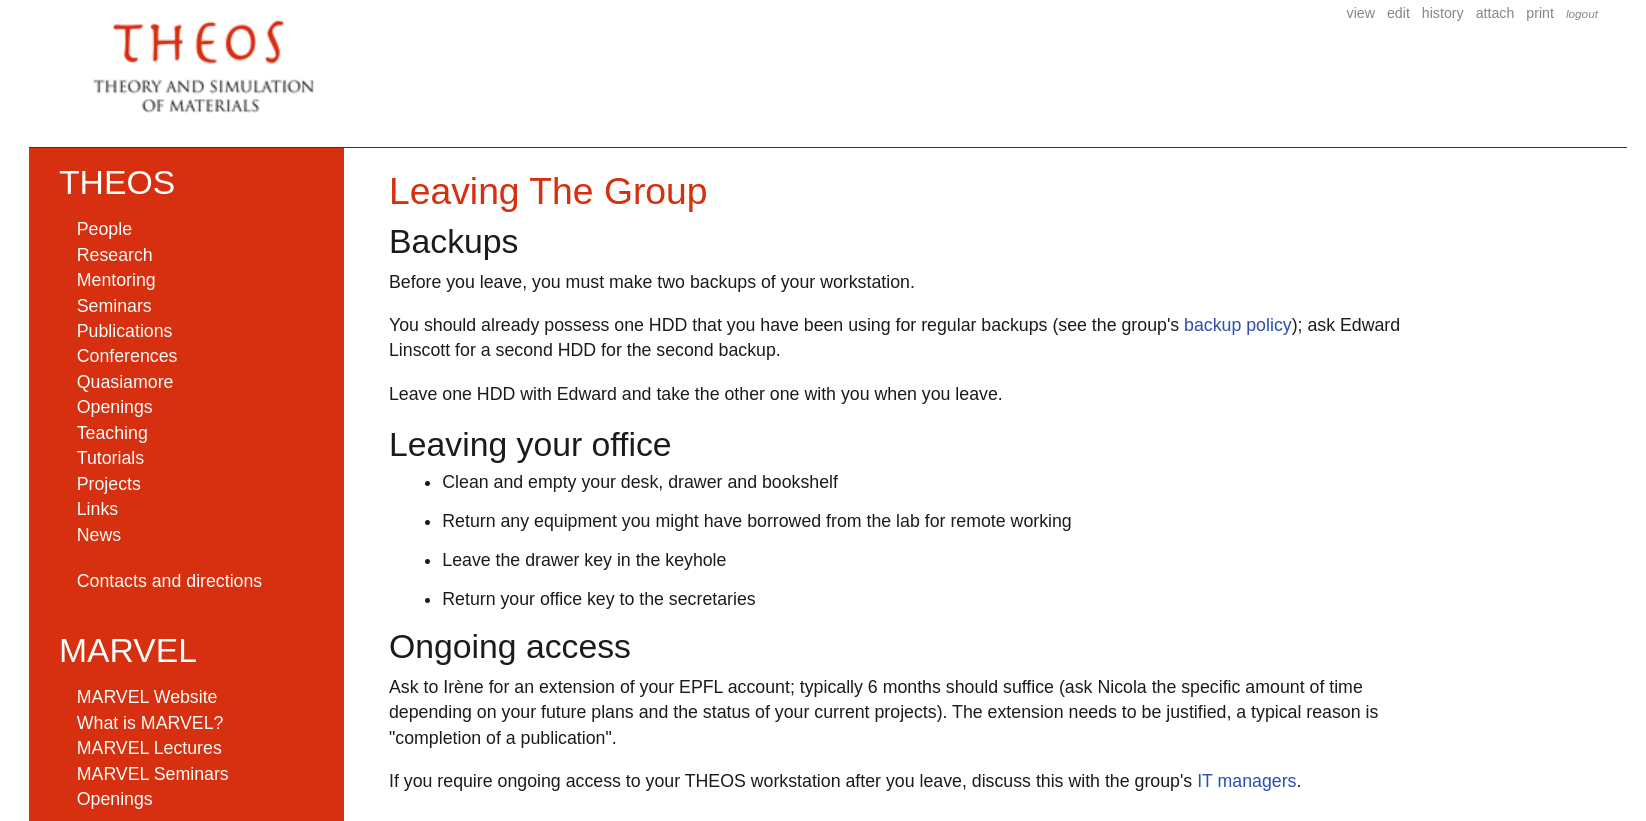
\includegraphics[width=0.9\textwidth]{figures/leaving_the_group.png}
\end{frame}

\frame{\titlepage}
% \frame{\titlepage}

% Preamble
% \begin{abstract}
%     From various discussions it has become clear that the standard DFT+\emph{U}+\emph{V} functional as developed and used at THEOS has several notable drawbacks. Chief among these is the fact that the corrections are applied to both spin channels equally. This is not a good idea when one spin channel is completely empty/filled and lying very far above/below the Fermi level, therefore not contributing to the value of $U$ but nevertheless being subjected to it. In these notes I review the findings of Linscott et al. 2018, and I explore the possibilities for a novel DFT+\emph{U}-inspired functional that does not apply the same value of $U$ to both spin channels, as well as the possibility of a correction that addresses static correlation error.
% \end{abstract}
% 
% \maketitle
% 
% \section{The problem}
% This discussion was inspired by the following results of Fatemeh Haddadi: for monolayers of CrI\textsubscript{3}, the unoccupied spin-down Hubbard bands are dramatically by a Hubbard correction. We guess that this should not happen\footnote{N.B. to properly determine this we ought to calculate spin-resolved response matrices; see the following section} because these bands are expected not to play a significant role in determining the value of $U$.
% 
% \begin{frame}{The problem}
% \begin{figure}[b!]
%     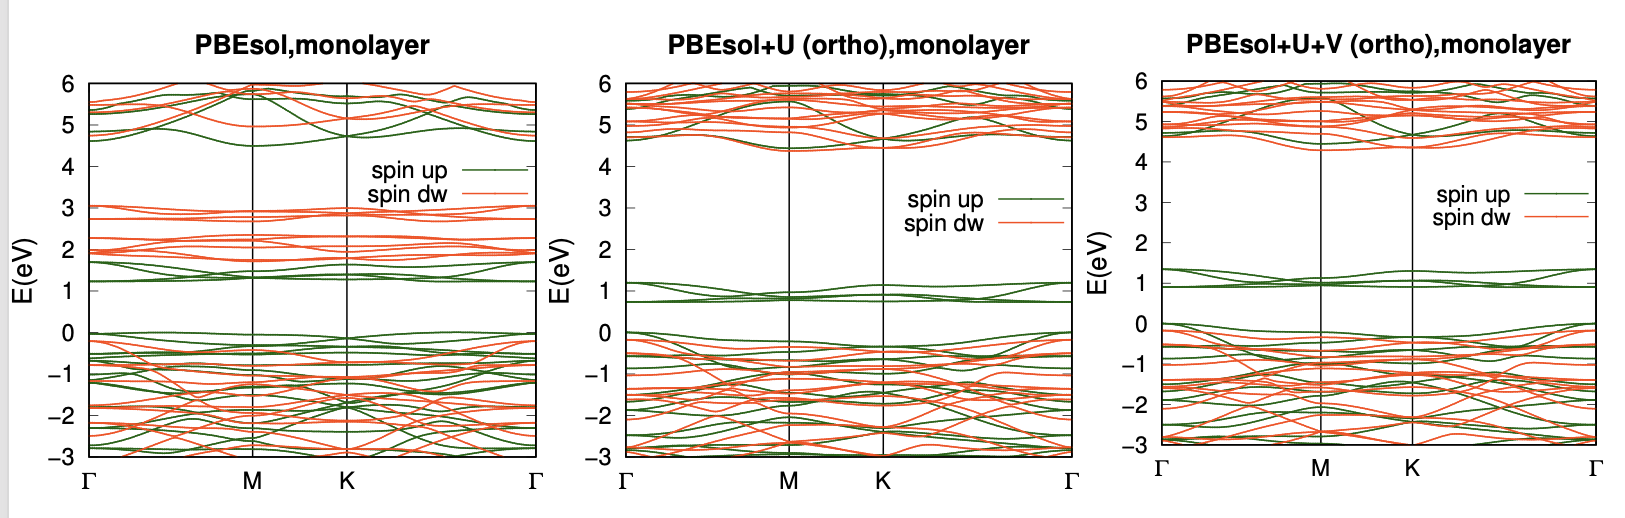
\includegraphics[width=\columnwidth]{figures/fig_haddadi_bs.png}
%     \caption{Band structure of a CrI\textsubscript{3} monolayer, as calculated with DFT, DFT+U, and DFT+U+V}
% \end{figure}
% \end{frame}
% 
% 
% \section{Lessons from Linscott et al. 2018}
% In a paper a few years ago, David O'Regan and I worked on a spin-resolved formulation of DFT+\emph{U} \cite{Linscott2018}. In this framework, all the matrices acquire an additional two spin indices e.g. the interacting and non-interacting response matrices are now
% %
% \begin{frame}{Spin-resolved linear response}
% \begin{equation}
%     \chi_{IJ\sigma\sigma'} = \frac{dn^{I\sigma}}{dv^{J\sigma'}_\mathrm{ext}}; \qquad
%     \chi^0_{IJ\sigma\sigma'} = \frac{dn^{I\sigma}}{dv^{J\sigma'}_\mathrm{KS}}
%     \label{eqn:spin_resolved_chi}
% \end{equation}
% %
% where now our external perturbing potential takes the form
% %
% \begin{equation}
%     dv^{I\sigma}_\mathrm{ext} = \alpha^\sigma \hat P^I = \alpha^\sigma \sum_m \ket{\varphi^I_m}\bra{\varphi^I_m}
%     \label{eqn:spin_resolved_v}
% \end{equation}
% \end{frame}
% 
% \begin{frame}{Results of spin-resolved linear response}
% \begin{align}
%     \chi^{\sigma\sigma'} = 
%     \begin{pmatrix}
%     -0.192 & 0.141 \\
%     0.141 & -0.214
%     \end{pmatrix};
%     \qquad
%     \chi_0^{\sigma\sigma'} = 
%     \begin{pmatrix}
%     -0.285 & 0.0 \\
%     0.0 & -0.226
%     \end{pmatrix}
% \end{align}
% %
% It follows that
% %
% \begin{align}
%     U^{\sigma\sigma'}
%     = \left(\chi_0^{-1} - \chi^{-1}\right)_{\sigma\sigma'}
%     =
%     \begin{pmatrix}
%         6.54 & 6.62 \\
%         6.62 & 4.61
%     \end{pmatrix}
%     _{\sigma\sigma'}
% \end{align}
% 
% N.B. with a spin-resolved matrix we can reconstruct other perturbations post-hoc e.g. conventional LR
% 
% \begin{equation}
%     dn = \sum_\sigma dn^\sigma = \sum_{\sigma}\left(\sum_{\sigma'} \chi^{\sigma\sigma'}dv^{\sigma'} \right) \stackrel{dv^\uparrow = dv^\downarrow = d\alpha}{\Longrightarrow} \chi = \frac{dn}{d\alpha} = \sum_{\sigma\sigma'} \chi_{\sigma\sigma'}
% \end{equation}
% 
% 
% \end{frame}
% %
% In order to construct our response matrices, we perturbed one spin channel at a time. To then connect these response matrices to $U$ and $J$ parameters you can derive the Dyson equation
% %
% \begin{equation}
%     U_{IJ\sigma\sigma'} = (\chi_0^{-1} - \chi^{-1})_{IJ\sigma\sigma'}
%     \label{eqn:spin_resolved_U}
% \end{equation}
% %
% However, we immediately encounter a problem when we try and marry this four-rank tensor with the idea of a scalar $U$ that corresponds to the curvature with respect to the \emph{total} occupancy of a particular Hubbard subspace; that is,
% %
% \begin{equation}
%     U^I = \frac{d^2E_\mathrm{Hxc}}{d(n^I)^2} = \frac{1}{2}\frac{d(v_\mathrm{Hxc}^\uparrow + v_\mathrm{Hxc}^\downarrow)}{d(n^{I\uparrow} + n^{I\downarrow})}
%     \label{eqn:U_as_curvature}
% \end{equation}
% %
% which we clearly cannot simplify to a nice expression involving response matrices. At this point in the paper, we resorted to using a contrived averaging scheme, because we wanted to stay loyal to this definition of $U$.
% 
% I propose the way forward is to do away with \cref{eqn:U_as_curvature}; that is, we should not try and calculate a curvature with respect to the \emph{total} occupancy of a subspace. Instead, we should be aiming to correct curvature with respect to the occupancy of subspaces, \emph{one spin channel at a time}. The natural way to do this is simply
% %
% \begin{equation}
%     U^{I\sigma} = \frac{d^2E_\mathrm{Hxc}}{d(n^{I\sigma})^2} = \frac{dv_\mathrm{Hxc}^{I\sigma}}{dn^{I\sigma}}
%     \label{eqn:Usigma_as_curvature}
% \end{equation}
% %
% We explored this approach Ref.~\cite{Linscott2018}. Various Hubbard parameters for hexahydrated transition metals (aqua-TMs) M(H\textsubscript{2}O)\textsubscript{6} and bulk MnO are tabulated in this fashion in \cref{tab:Udet_metal}, labelled ``$1 \times 1$". Also shown in this table are parameters calculated via conventional linear response, labelled ``scalar". There are a number of important observations we can make.
% 
% \begin{table}[t!]
%     \centering
%     \caption{Values of $U$ and $J$ (eV) for aqua-TMs and a spin-up manganese atom of MnO, calculated using the various linear response schemes introduced in \cite{Linscott2018}. Note that we struggled to get the Fe\textsuperscript{3+} calculation to converge (hence the missing data) and Co\textsuperscript{3+} is the only one of these systems with a low-spin (i.e. singlet) ground state (hence $U^\uparrow = U^\downarrow$ for that system).}
%     \label{tab:Udet_metal}
%     \footnotesize
%     \begin{tabular}{m{1.5cm} |
%             d @{$\,\pm$}d |
%             d @{$\,\pm$}d |
%             d @{$\,\pm$}d
%             d @{$\,\pm$}d}
%         \hline
%         \multicolumn{1}{c |}{\multirow{2}{*}{metal}}
%          & \multicolumn{2}{c |}{scalar}
%          & \multicolumn{2}{c |}{averaged $1\times1$}
%          & \multicolumn{4}{c}{$1\times1$}            \\
%          & \multicolumn{2}{c|}{$U$}
%          & \multicolumn{2}{c|}{$U$}
%          & \multicolumn{2}{c}{$U^\uparrow$}
%          & \multicolumn{2}{c}{$U^\downarrow$}        \\
%         \hline
%         \input{tab_Udet_metal_truncated}
%         \hline
%         \input{tab_Udet_MnO_opium_metal_truncated}
%         \hline
%     \end{tabular}
% \end{table}
% 
% Firstly, this spin-resolved approach yields Hubbard parameters are screened by the opposite spin channel (that is, by neglecting $\chi_{II\downarrow\uparrow}$ this response is absorbed into $U^{I\sigma}$). This typically resulted in smaller Hubbard parameters, especially for the low-spin aqua-Co\textsuperscript{3+}, where inter-spin-channel screening will be large.
% 
% Secondly, if the given spin channel has a small response (i.e. if it lies far from the Fermi level) then a small response results in a \emph{large} $U$! This is especailly noticeable in the values of $U^{\uparrow}$ for the late aqua-TMs.\footnote{We did't see the same effect for $U^\downarrow$ of the early aqua-TMs because $n^\downarrow$ never goes to zero for these systems, whereas $n^\uparrow$ reaches the maximum possible value for Mn\textsuperscript{2+} and heavier -- likely due to some projection-related subtleties. See Figure 4 of Ref.~\cite{Linscott2018} for details.} For copper it is even large and negative! We can explain this behaviour because in \cref{eqn:Usigma_as_curvature}, if we induce a slight change in the occupancy of this subspace it will bring about a very large change in the Hartree-plus-xc potential.
% 
% These large Hubbard parameters obviously have implications for quasiparticle energies, which will likely suffer.\footnote{You can see this in Table V of our paper, where the quasiparticle energies for the late aqua-TMs are grossly overestimated.} This should not come as too much of a surprise given that the Hubbard parameters were constructed without reference to quasiparticle energies.
% 
% N.B. this is no different from the behaviour one would get if we did conventional DFT\,+\,\emph{U} on a system with a completely filled or empty $3d$ subshell (e.g. ZnO). By separating the spin channels we have restricted things for ourselves even more, because we need to avoid systems where $n^\uparrow$ is not totally filled (and in principle $n^\downarrow$ not totally empty). This is obviously too restrictive to be of practical use.\footnote{That said, as we saw for the early aqua-TMs depending on the precise definition of our Hubbard projectors it might not be an issue}
% 
% \section{DFT\,+\,\emph{U}\,(+\,\emph{J})}
% In order to inspire the design of functionals, it is worthwhile reviewing the properties of the conventional DFT\,+\,\emph{U}+\,\emph{J} functional \cite{Himmetoglu2011a,Himmetoglu2014a}:
% %
\begin{frame}
    \begin{align}
        E_{U} = & \sum_{I\sigma m m'} \frac{U^I}{2} \left(n^{I\sigma}_{mm'} (\delta_{m'm} - n^{I\sigma}_{m'm})\right) \label{eqn:u_correction}                              \\
        E_{J} = & \sum_{I\sigma m m'} \frac{J^I}{2} \left( n^{I\sigma}_{mm'} n^{I-\sigma}_{m'm} - 2\delta_{\sigma \sigma_\mathrm{min}}\delta_{mm'} n^{I\sigma}_{m'm}\right)
        \label{eqn:j_correction}
    \end{align}
\end{frame}
% %
% Now, let us consider the He\textsuperscript{$x+$} atom for $x = [0, 2]$, with a Hubbard correction applied to the $1s$ orbital.\footnote{Actually, all of the following is more general, and applies to any orbital that is an eigenvector of $n^\sigma_{mm'}$ for both spin channels.} The $+U$ correction to this subspace is pictured in \cref{fig:u_correction}. Note that\dots
% 

\begin{frame}{Rethinking inter-spin corrections: He$\textsuperscript{\emph{x}+}$}

    \renewcommand{\figurename}{}
    \vspace{-2ex}
    \begin{columns}
        \column{0.35\linewidth}

        \begin{figure}
            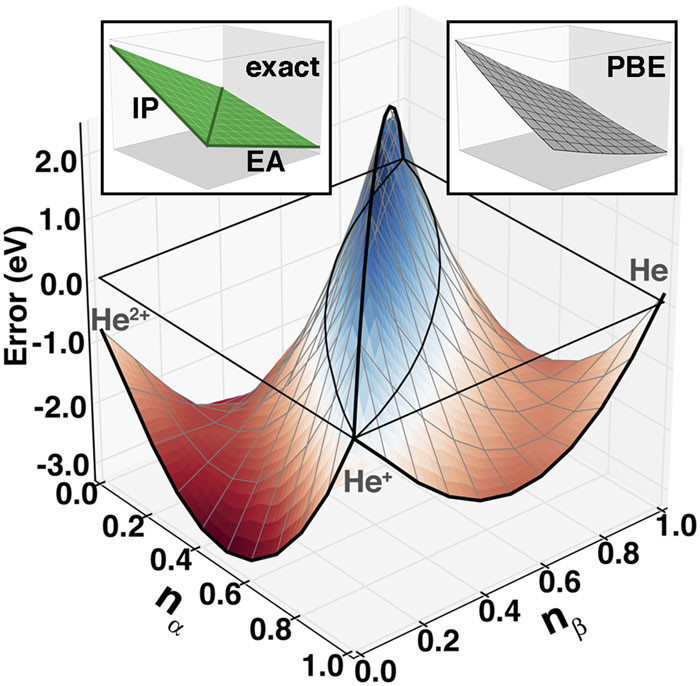
\includegraphics[width=\columnwidth]{figures/fig_bajaj_2d_pwl.jpeg}
            \caption{PBE error}
        \end{figure}

        \column{0.3\linewidth}
        \begin{figure}[h!]
            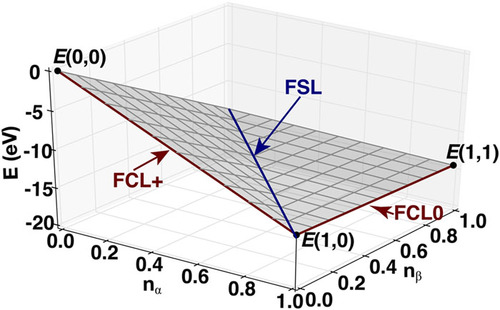
\includegraphics[width=\columnwidth]{figures/fig_bajaj_abstracted_2d_pwl.jpg}
            \caption{the flat plane}
        \end{figure}

        \vspace{-6ex}
        \begin{figure}
            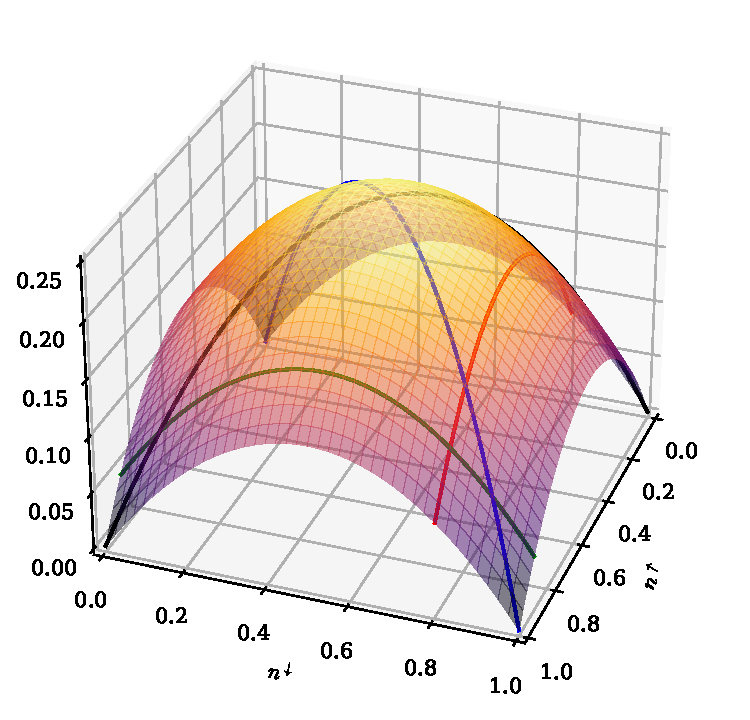
\includegraphics[width=\columnwidth]{figures/u_correction_with_paths.pdf}
            \caption{the $+U$ correction}
        \end{figure}

        \column{0.3\linewidth}

        \begin{figure}
            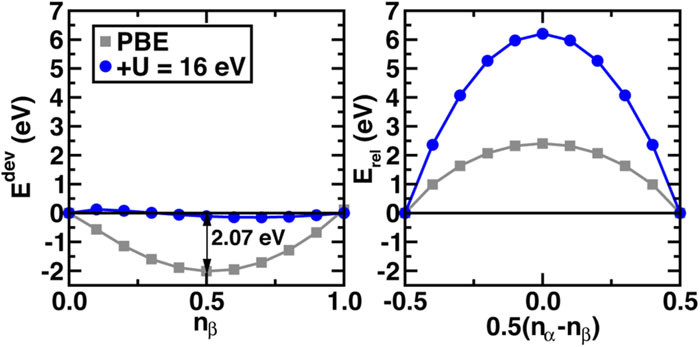
\includegraphics[width=\columnwidth]{figures/fig_bajaj_u_worsens_sce.jpeg}
            \caption{error along $n = 1$}
        \end{figure}

        \vspace{-6ex}
        \begin{figure}
            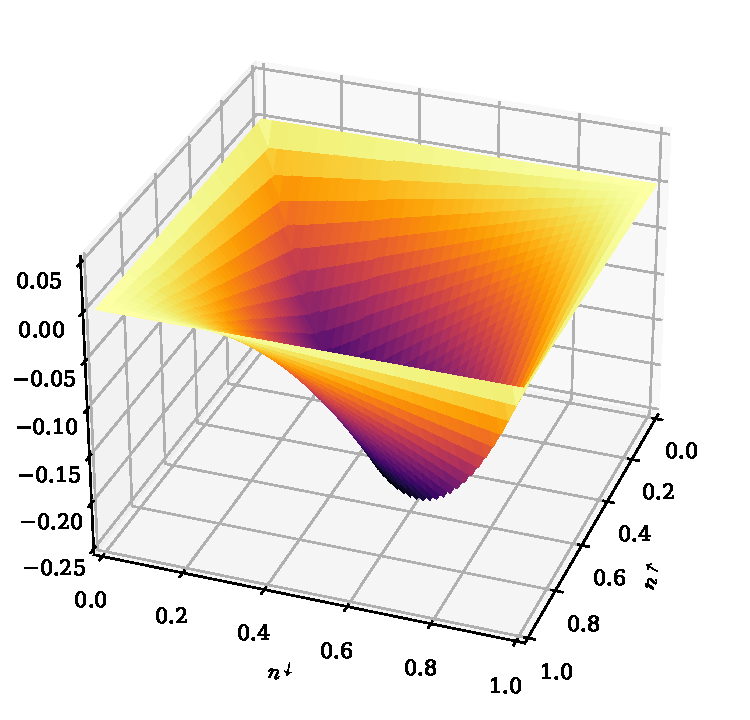
\includegraphics[width=\columnwidth]{figures/j_correction.pdf}
            \caption{the $+J$ correction}
        \end{figure}

    \end{columns}

    \vspace{-2ex}
    \blfootcite{Bajaj2017}
\end{frame}

\begin{frame}{The +\,\emph{U} correction}
    \begin{columns}
        \column{0.6\linewidth}
        \begin{figure}[h!]
            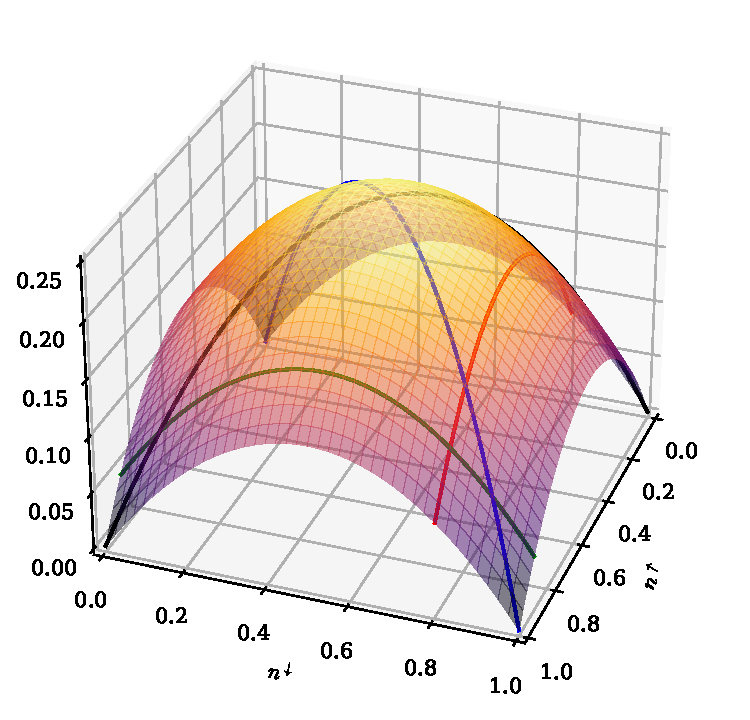
\includegraphics[width=\columnwidth]{figures/u_correction_with_paths.pdf}
            \caption{$E_{U}(n^\uparrow,n^\downarrow)$}
            \label{fig:u_correction_with_paths}
        \end{figure}
        \column{0.35\linewidth}
        \small
        \begin{subequations}
            \begin{align}
                \left.\frac{\partial^2E_{U}}{\partial n^{\uparrow 2}}\right|_{n^\downarrow} & = -U \qquad \text{(red)}             \\
                \left.\frac{\partial^2E_{U}}{\partial n^{\downarrow 2}}\right|_{n^\uparrow} & = -U \qquad \text{(green)}           \\
                \left.\frac{\partial^2E_{U}}{\partial n^2}\right|_{\mu}                     & = -\frac{U}{2} \qquad \text{(blue)}  \\
                \left.\frac{\partial^2E_{U}}{\partial \mu^2 }\right|_{n}                    & = -\frac{U}{2} \qquad \text{(black)}
            \end{align}
        \end{subequations}
    \end{columns}
    %
\end{frame}
% % 
% % The $+U$ correction introduces a spin-symmetric curvature with respect to $n^\sigma$, but also adds curvature with respect to $\mu$. For semi-local functionals $\frac{d^2E}{d\mu^2}$ is already erroneously \emph{concave}, and thus $+U$ corrections worsen static correlation error \cite{Bajaj2017}.
% % 
\begin{frame}{The +\,\emph{J} correction}
    \begin{columns}
        \column{0.6\linewidth}
        \begin{figure}[h!]
            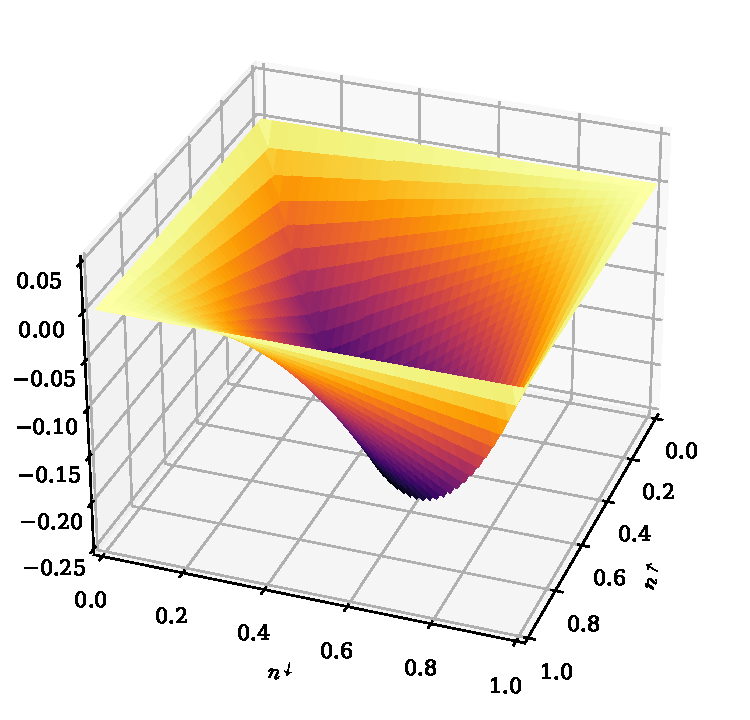
\includegraphics[width=\columnwidth]{figures/j_correction.pdf}
            \caption{$E_{J}(n^\uparrow,n^\downarrow)$}
            \label{fig:j_correction}
        \end{figure}
        \column{0.35\linewidth}
        %
        \footnotesize
        \begin{subequations}
            \begin{align}
                \left.\frac{\partial^2E_{J}}{\partial n^2}\right|_{\mu}                     & = \frac{J}{2}                                 \\
                \left.\frac{\partial^2E_{J}}{\partial\mu^2}\right|_{n}                      & = -\frac{J}{2} \qquad \text{ for } \mu \neq 0 \\
                \left.\frac{\partial^2E_{J}}{\partial n^{\uparrow 2}}\right|_{n^\downarrow} & = 0                                           \\
                \left.\frac{\partial^2E_{J}}{\partial n^{\downarrow 2}}\right|_{n^\uparrow} & = 0
            \end{align}
        \end{subequations}
    \end{columns}
\end{frame}
% % 
% % \subsection{Should we use $U$ or $U_\mathrm{eff} = U - J$?}
% % 
% % \begin{figure}[h!]
% %     \begin{subfigure}[b]{0.4\columnwidth}
% %         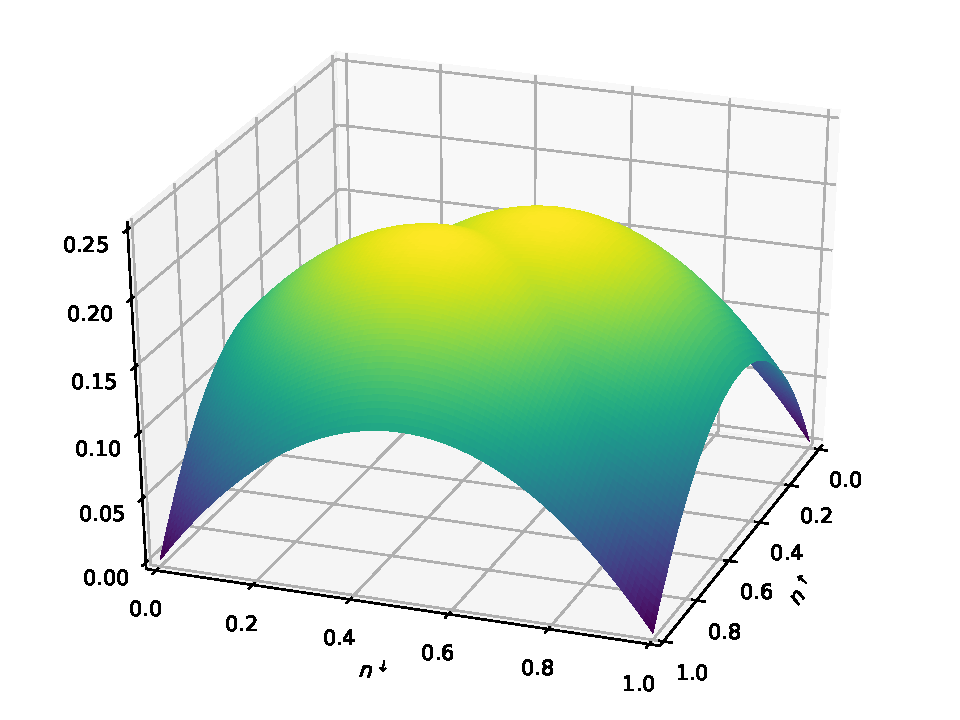
\includegraphics[width=\columnwidth]{figures/u_j_correction.pdf}
% %         \caption{with a $E_U$ prefactor of $U - J$}
% %         \label{fig:u_j_correction}
% %     \end{subfigure}
% %     \begin{subfigure}[b]{0.4\columnwidth}
% %         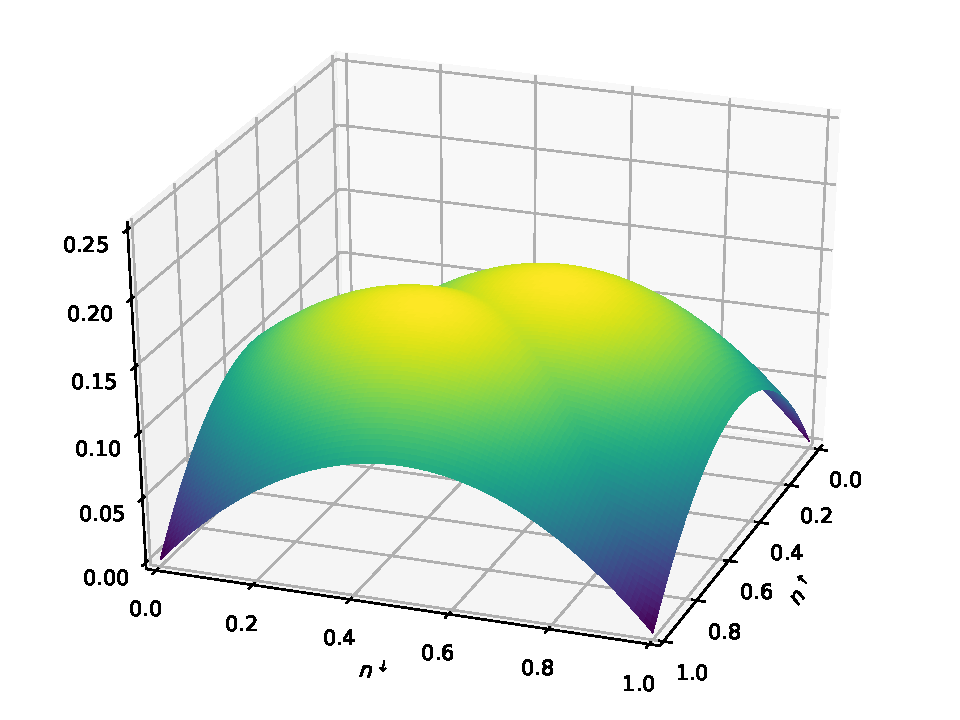
\includegraphics[width=\columnwidth]{figures/ueff_j_correction.pdf}
% %         \caption{with a $E_U$ prefactor of $U$}
% %         \label{fig:ueff_j_correction}
% %     \end{subfigure}
% %     % \begin{subfigure}[b]{0.4\columnwidth}
% %     %     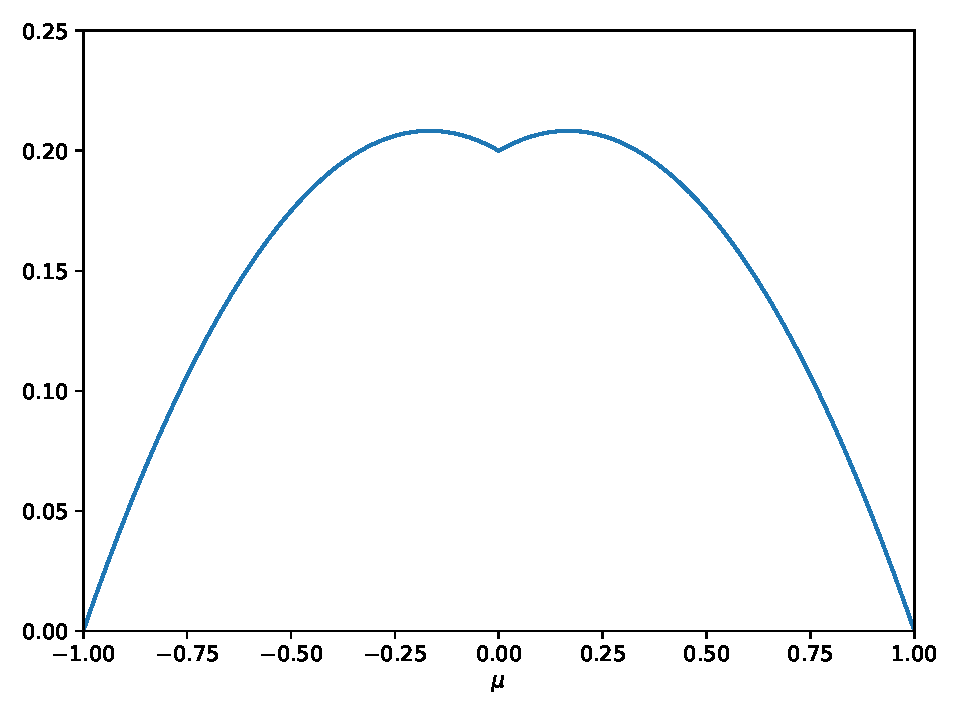
\includegraphics[width=\columnwidth]{figures/u_j_correction_2d.pdf}
% %     %     \caption{cross-section of \cref{fig:u_j_correction} along $n=1$}
% %     %     \label{fig:u_j_correction_2d}
% %     % \end{subfigure}
% %     % \begin{subfigure}[b]{0.4\columnwidth}
% %     %     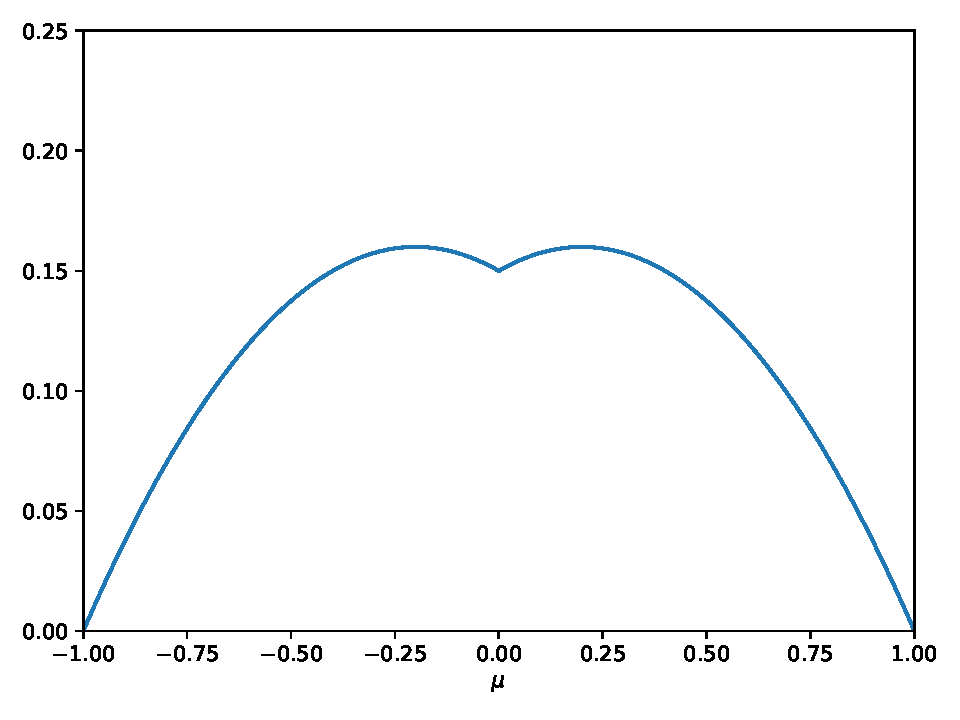
\includegraphics[width=\columnwidth]{figures/ueff_j_correction_2d.pdf}
% %     %     \caption{cross-section of \cref{fig:ueff_j_correction} along $n=1$}
% %     %     \label{fig:ueff_j_correction_2d}
% %     % \end{subfigure}
% %     \caption{The corrective surface $E_U(n^\uparrow, n^\downarrow) + E_J(n^\uparrow, n^\downarrow)$, for $J = 0.2U$}
% %     \label{fig:u_vs_ueff}
% % \end{figure}
% % %
% % \noindent Often the prefactor to the +\,\emph{U} correction is rendered as $U_\mathrm{eff} = U - J$. In this framework, if we want to apply some value for $J$ to our system we should simultaneously reduce the prefactor of the +\,\emph{U} correction by the same amount.
% % 
\begin{frame}{The combined correction}
    \footnotesize
    \begin{columns}
        \column{0.45\linewidth}
        $U_\mathrm{eff} = U - J$:
        \begin{subequations}
            \begin{align}
                \left.\frac{\partial^2}{\partial n^2}\right|_{\mu} (E_{U_\mathrm{eff}} + E_J)                     & = -\frac{U-2J}{2}                            \nonumber  \\
                \left.\frac{\partial^2}{\partial \mu^2}\right|_{n} (E_{U_\mathrm{eff}} + E_J)                     & = -\frac{U}{2} \qquad \text{ for } \mu \neq 0 \nonumber \\
                \left.\frac{\partial^2}{\partial n^{\uparrow 2}}\right|_{n^\downarrow} (E_{U_\mathrm{eff}} + E_J) & = -(U - J) \qquad \text{ for } \mu \neq 0     \nonumber \\
                \left.\frac{\partial^2}{\partial n^{\downarrow 2}}\right|_{n^\uparrow} (E_{U_\mathrm{eff}} + E_J) & = -(U - J) \qquad \text{ for } \mu \neq 0\nonumber
            \end{align}
            \label{eqn:2nd_derivatives_ueff_plus_j}
        \end{subequations}
        \column{0.45\linewidth}
        $U_\mathrm{eff} = U$:
        \begin{subequations}
            \begin{align}
                \left.\frac{\partial^2}{\partial n^2}\right|_{\mu} (E_{U} + E_J)                     & = -\frac{U-J}{2}                                \nonumber \\
                \left.\frac{\partial^2}{\partial \mu^2}\right|_{n} (E_{U} + E_J)                     & = -\frac{U+J}{2} \qquad \text{ for } \mu \neq 0 \nonumber \\
                \left.\frac{\partial^2}{\partial n^{\uparrow 2}}\right|_{n^\downarrow} (E_{U} + E_J) & = -U \qquad \text{ for } \mu \neq 0             \nonumber \\
                \left.\frac{\partial^2}{\partial n^{\downarrow 2}}\right|_{n^\uparrow} (E_{U} + E_J) & = -U \qquad \text{ for } \mu \neq 0\nonumber
            \end{align}%
            \label{eqn:2nd_derivatives_u_plus_j}%
        \end{subequations}%
    \end{columns}
    %
\end{frame}
% % %
% % These two approaches are also plotted in \cref{fig:u_vs_ueff}. We can see immediately there are a number of issues with using $U_\mathrm{eff}$. All bar one of these curvature corrections is parametrised by a mix of $U$ and $J$ -- and bizarrely the one that is parametrised solely by $U$ is the curvature with respect to $\mu$!
% % 
% % Using $U$ rather than $U_\mathrm{eff}$ (\cref{eqn:2nd_derivatives_u_plus_j}) is not much better, with the curvature with respect to $n$ and $\mu$ being a function of both $U$ and $J$. At least in this scheme, the derivatives with respect to $n^\sigma$ are parametrised by $U$ alone. Thus \textbf{using $U$ rather than $U_\mathrm{eff}$ is a better (if imperfect) choice} when performing DFT\,+\,$U$\,+\,$J$.
% % 
% % \subsection{What to do with the minority spin term?}
% \begin{frame}{Excluding the minority spin}
%     \footnotesize
%     \vspace{-1em}
%     \begin{align}
%         E_{J} = & \sum_{I\sigma m m'} \frac{J^I}{2} \left( n^{I\sigma}_{mm'} n^{I-\sigma}_{m'm} - 2\delta_{\sigma \sigma_\mathrm{min}}\delta_{mm'} n^{I\sigma}_{m'm}\right)
%         \label{eqn:j_correction}
%     \end{align}
%     \begin{figure}
%         \begin{subfigure}[b]{0.4\columnwidth}
%             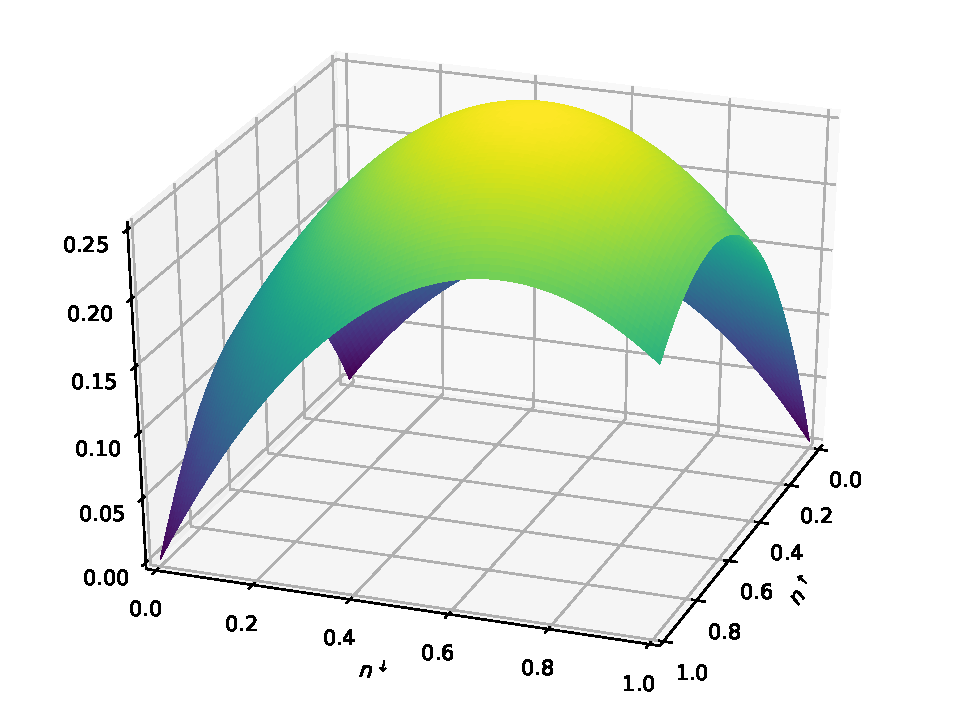
\includegraphics[width=\columnwidth]{figures/u_jnomin_correction.pdf}
%             \caption{with a $E_U$ prefactor of $U - J$}
%             \label{fig:u_jnomin_correction}
%         \end{subfigure}
%         \begin{subfigure}[b]{0.4\columnwidth}
%             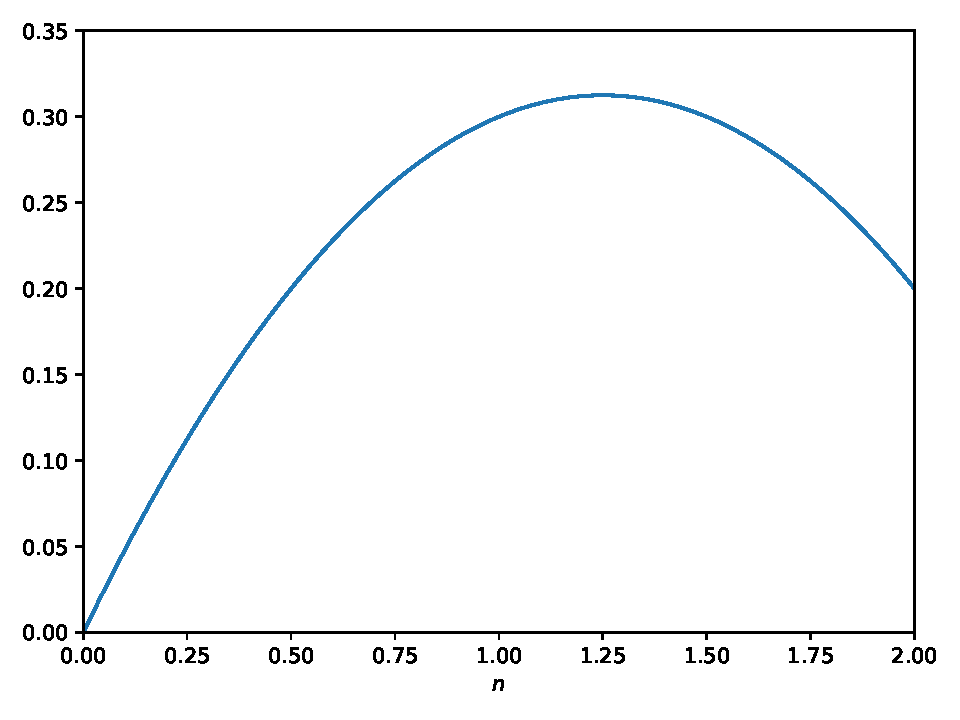
\includegraphics[width=\columnwidth]{figures/u_jnomin_correction_2d.pdf}
%             \caption{Cross-section along $\mu=0$}
%             \label{fig:u_jnomin_correction_2d}
%         \end{subfigure}
%         \caption{The corrective surface $E_U(n^\uparrow, n^\downarrow) + E_J(n^\uparrow, n^\downarrow)$, for $J = 0.2U$, where $E_J$ does not include the minority spin term.}
%         \label{fig:j_vs_jnomin}
%     \end{figure}
% \end{frame}
% 
% Sometimes the ``minority spin term" in the $+J$ correction\footnote{that is, the second term in \cref{eqn:j_correction}} is dropped because it can lead to numerical difficulties. However, this leads to a much more grevious error: the $+J$ correction without this term is non-vanishing when both spin channels are filled (see \cref{fig:j_vs_jnomin}). This is the case regardless of whether the Hubbard correction prefactor is $U$ or $U_\mathrm{eff} = U - J$.
% 
% The general philosophy of Hubbard corrections is that we trust DFT to provide reliable energies at integer numbers of electrons,\footnote{For the moment I will be vague as to what occupancies I am talking about, although it's always worth keeping in mind that local occpuancies $n = \trace{n^{\sigma}_{mm'}}$ of Hubbard subspaces are very different from the total occupancy of the entire system $N$.} and any correction to the DFT energy should vanish at these points. It follows that \textbf{this minority spin term must not be dropped} and instead these numerical difficulties should be tolerated or somehow overcome.
% 
% \section{Criteria for sensible Hubbard-like corrections}
% \noindent The goal of this work is to devise a new Hubbard-like correction to address self-interaction error (SIE) and static correlation error (SCE). At this point there are several philosophical choices one can make. Based on our above study of the DFT\,+\,$U$\,+\,$J$ here are the properties I would like my functional to possess:
% 
\begin{frame}{Rethinking inter-spin corrections}
    \begin{align}
        E_{U} = & \sum_{I\sigma m m'} \frac{U^I}{2} \left(n^{I\sigma}_{mm'} (\delta_{m'm} - n^{I\sigma}_{m'm})\right) \label{eqn:u_correction}                              \\
        E_{J} = & \sum_{I\sigma m m'} \frac{J^I}{2} \left( n^{I\sigma}_{mm'} n^{I-\sigma}_{m'm} - 2\delta_{\sigma \sigma_\mathrm{min}}\delta_{mm'} n^{I\sigma}_{m'm}\right)
        \label{eqn:j_correction}
    \end{align}
    Observations on conventional DFT\,+\,$U$ and DFT\,+\,$U$\,+\,$J$
    \begin{itemize}
        \item the correction is not the right shape
        \item lots of inter-dependence
        \item $U^I$ not $U^I_\mathrm{eff} = U^I - J^I$
        \item minority $J$ term is important
    \end{itemize}

    Principles for designing a new correction
    \begin{enumerate}
        \item vanishing at integer occupancies
        \item decouple our treatment of SIE and SCE
        \item different $U$ correction for each spin channel
    \end{enumerate}
\end{frame}
% %
% Finally, the correction I will construct will simply be designed to fit the shape of the errors we are trying to address, without reference to some sort of physical model. We all know that historically the Hubbard correction was (somewhat arbitrarily) derived from the Hubbard model. I do not think this is the right approach. Instead, I believe that it is much better to be pragmatic, and, in the spirit of Matteo's 2005 paper, simply choose a corrective term that best addresses the errors we are trying to correct: that is (a) quadratic corrections to the energy in terms of the occupancies of individual orbitals and (b) quadratic corrections to the energy in terms of the magnetic moment of individual orbitals.
% 
% \section{The novel functionals}
% \subsection{A novel correction for SIE}
% Here is my first proposed energy correction for our \emph{1s} system, first attempting to address self-interaction error:
% 
\begin{frame}{Correction to SIE}
    \begin{equation}
        % E_1(\{U^\sigma\}, \{n^\sigma\}) = \sum_\sigma \frac{U^\sigma}{4} \left(|\tilde n| + \tilde n(1 - 2n^\sigma)\right)
        E_1(\{U^\sigma\}, \{n^\sigma\}) =
        \sum_\sigma \frac{U^\sigma}{2} \left(n^\uparrow + n^\downarrow - 1\right) \times
        \begin{cases}
            -n^\sigma    & n < 1 \\
            1 - n^\sigma & n > 1
        \end{cases}
        \label{eqn:novel_u_correction}
    \end{equation}
    %
    \begin{figure}[t!]
        \begin{subfigure}[b]{0.4\columnwidth}
            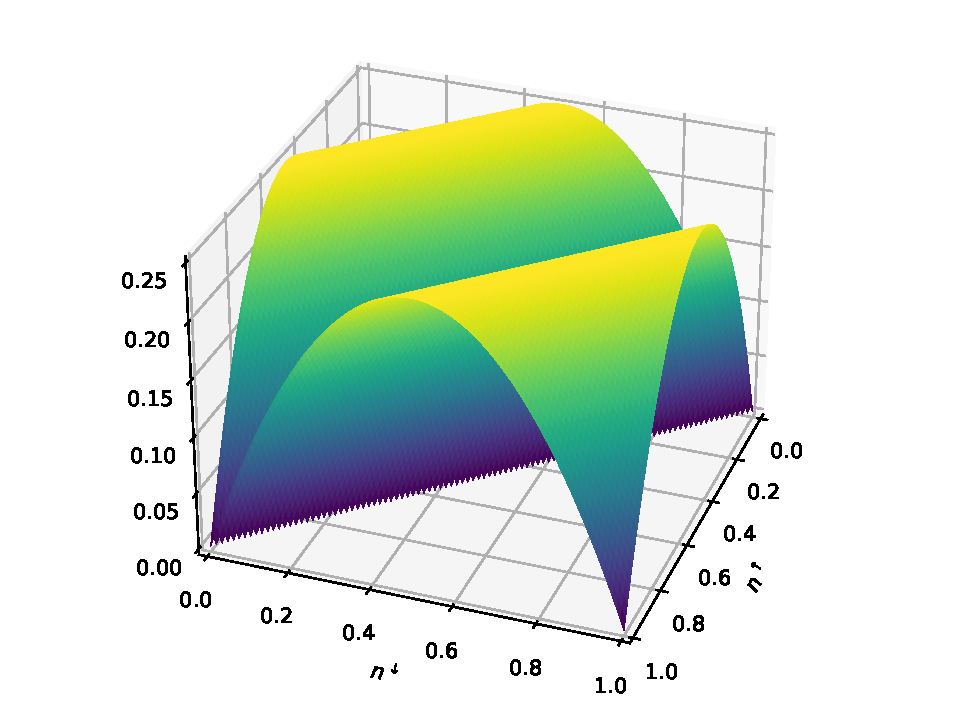
\includegraphics[width=\columnwidth]{figures/novel_u_correction_equal.pdf}
            \caption{$U^\uparrow = U^\downarrow$}
        \end{subfigure}
        \begin{subfigure}[b]{0.4\columnwidth}
            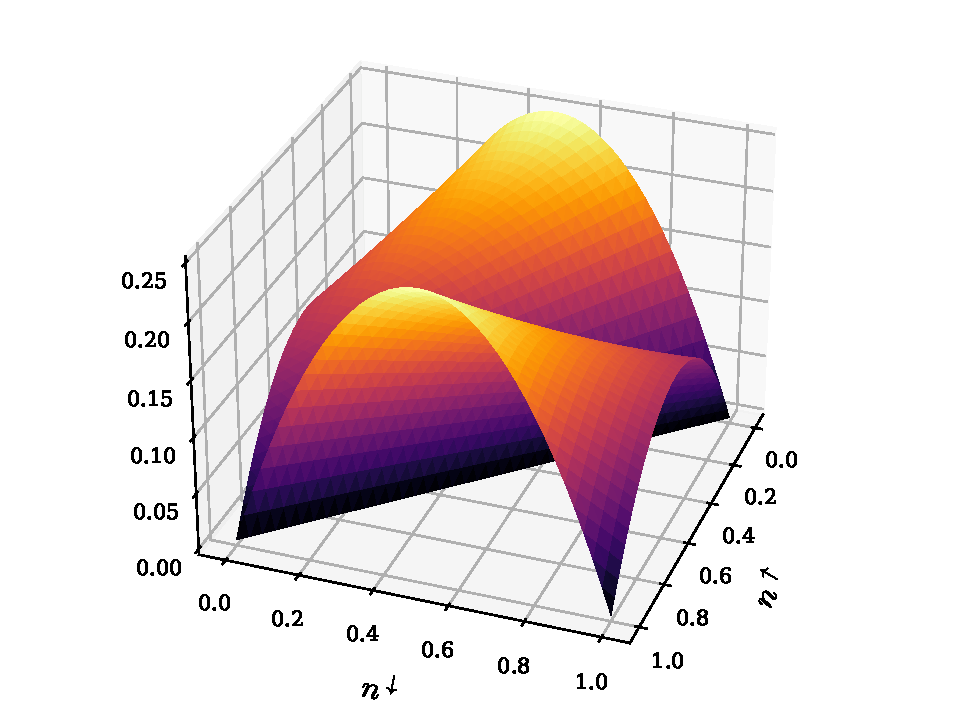
\includegraphics[width=\columnwidth]{figures/novel_u_correction.pdf}
            \caption{$U^\uparrow = U^\downarrow/2$}
        \end{subfigure}
    \end{figure}
\end{frame}
% % %
% % The notable properties of this functional are as follows
% % %
\begin{frame}{Correction to SIE}
    \begin{columns}
        \column{0.38\linewidth}
        \centering
        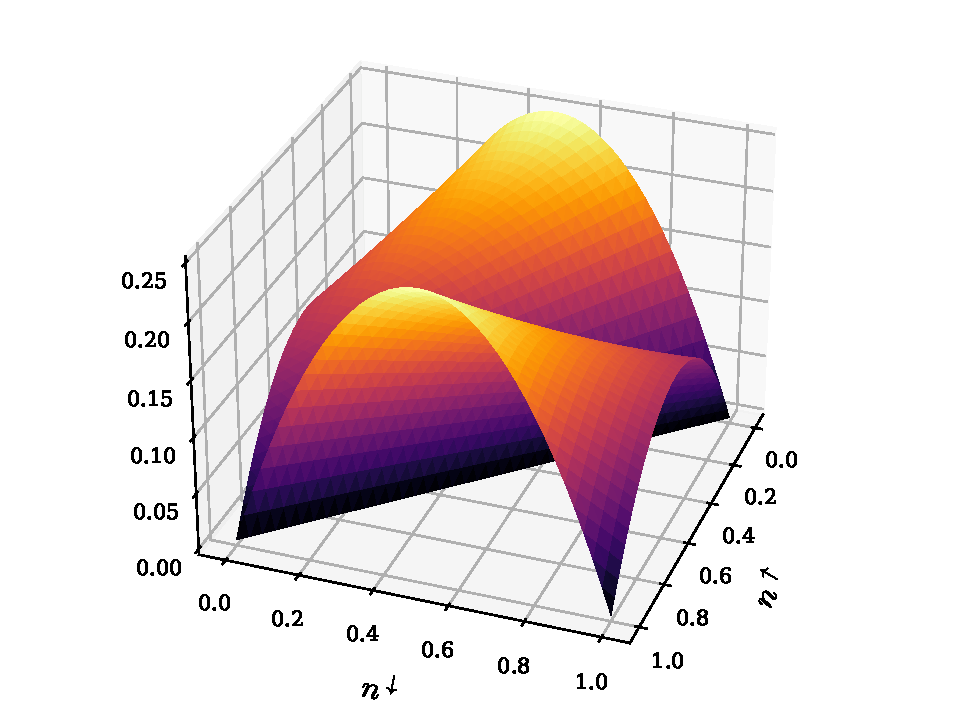
\includegraphics[width=1\columnwidth]{figures/novel_u_correction.pdf}
        \column{0.58\linewidth}
        \footnotesize
        \begin{enumerate}
            \item it is zero for integer numbers of electrons
            \item the curvature with respect to $n^\sigma$ is entirely controlled by $U^\sigma$, i.e.
                  \begin{equation}
                      \left.\frac{\partial^2 E_1}{\partial n^{\sigma 2}}\right|_{n^{-\sigma}} = - U^\sigma
                  \end{equation}
            \item the curvature with respect to $\mu$ is \emph{untouched} by this correction
                  \begin{equation}
                      \left.\frac{\partial^2 E_1}{\partial \mu^{2}}\right|_{n} = 0
                  \end{equation}
                  which would imply that this correction will selectively address SIE and not SCE
            \item the curvature with respect to the total occupancy $n = n^\uparrow + n^\downarrow$ is given by the average
                  \begin{equation}
                      \left.\frac{\partial^2 E_1}{\partial n^{2}}\right|_{\mu} = -\frac{U^\uparrow + U^\downarrow}{2}
                  \end{equation}
                  % I would argue that this curvature is less important (after all, derivatives with respect to $n^\sigma$ not $n$ give rise to the eigenenergies $\varepsilon^\sigma$) but nevertheless it is comforting that this second derivative is (a) constant everywhere and (b) is an intuitive value
        \end{enumerate}
    \end{columns}
\end{frame}
% % %
% % Of course, we do now have a discontinuity at $\tilde n = 0$. It remains to be seen if this will lead to numerical difficulties. It is not possible to construct this functional without this discontinuity while retaining the above properties.
% % 
% % % In order to generalise \cref{eqn:novel_u_correction} to a multi-orbital Hubbard site, I imagine the path forward is to work with the set of orbitals that diagonalise $n_{mm'}$, but I need to give this more thought as there are some subtleties.\footnote{e.g. $n_{mm'}$, $n_{mm'}^\uparrow$, and $n_{mm'}^\downarrow$ will diagonalised by different sets of orbitals}
% % %If $\{\ket{\varphi_i}\}$ is the set of orbitals that diagonalise $n_{mm'}$ then
% % 
\begin{frame}{Correction to SIE}
    The resulting potential from this energy correction is given by $\hat v^\sigma_1 = v^\sigma_1(n^\uparrow_i, n^\downarrow_i) \ket{i}\bra{i}$ where
    %
    \begin{align}
        v^\sigma_1(n^\uparrow, n^\downarrow)
        % = -\frac{\tilde n U^\sigma}{2} + \sum_{\sigma'} \frac{U^{\sigma'}}{4} \left[\frac{|\tilde n|}{\tilde n} + 1 - 2n^{\sigma'}\right]
        = &
        \begin{cases}
            U^\sigma\left(\frac{1}{2} - n^\sigma\right)
            + \left(1 - n^{-\sigma}\right)
            \frac{U^\uparrow + U^\downarrow}{2}
             & n > 1
            \\
            U^\sigma\left(\frac{1}{2} - n^\sigma\right)
            - n^{-\sigma}
            \frac{U^\uparrow + U^\downarrow}{2}
             & n < 1
        \end{cases}
        \label{eqn:novel_u_potential}
    \end{align}
    \begin{figure}[t!]
        \begin{subfigure}[b]{0.3\columnwidth}
            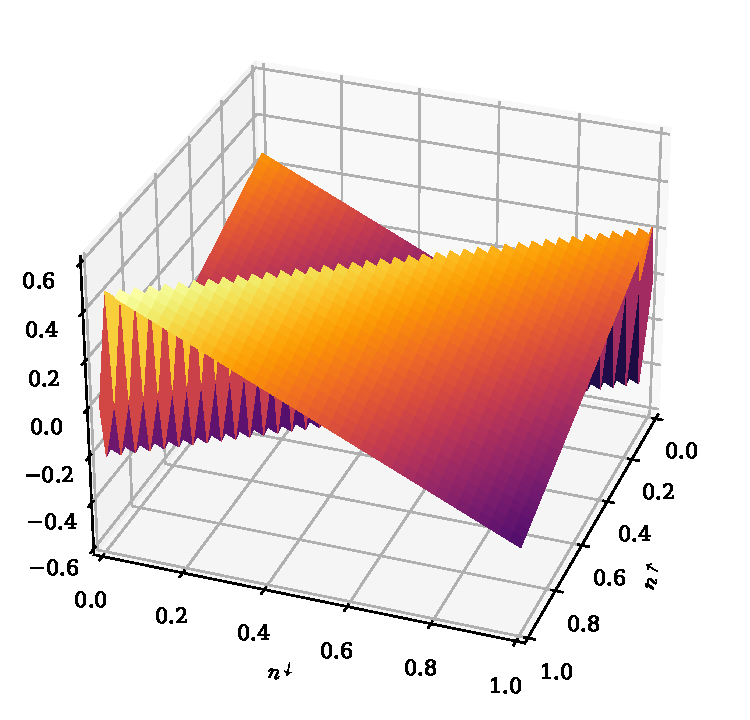
\includegraphics[width=\columnwidth]{figures/novel_u_potential.pdf}
            \caption{}
            \label{fig:novel_u_potential}
        \end{subfigure}
        \begin{subfigure}[b]{0.3\columnwidth}
            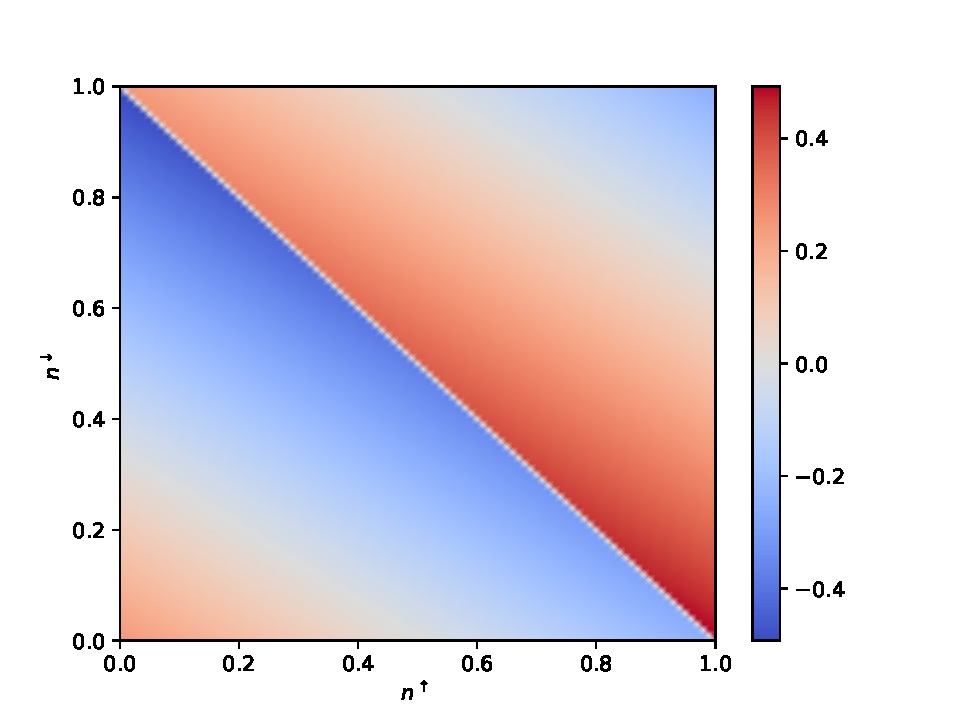
\includegraphics[width=\columnwidth]{figures/novel_u_potential_2d.pdf}
            \caption{}
            \label{fig:novel_u_potential_2d}
        \end{subfigure}
        \caption{my proposed potential correction $v^\uparrow_1(\{U^\sigma\}, \{n^\sigma\})$ for addressing SIE, with $U^\downarrow = 2 U^\uparrow$}
    \end{figure}

\end{frame}
% % %
% % This is plotted in \cref{fig:novel_u_potential,fig:novel_u_potential_2d}. The first term in this correction is very familiar -- it is simply the conventional +\emph{U} potential $\hat v = \sum_{i\sigma} U (\frac{1}{2} - n^\sigma_i)\ket{i}\bra{i}$ with a spin-dependent $U$! The second term is novel.
% % 
% % \subsection{A novel correction for SCE}
% % Here is my second proposed energy correction for our \emph{1s} system, now attempting to address static correlation error:
% % %
\begin{frame}{Correction to SCE}
    \vspace{-1em}
    \begin{equation}
        E_2(K, \{n^\sigma\}) % = & \frac{K}{4}\left[(n^\uparrow-n^\downarrow)^2-(|\tilde n|-1)^2\right] \nonumber \\
        % = & \frac{K}{4}\left[(n^\uparrow)^2 - 2n^\uparrow n^\downarrow + (n^\downarrow)^2-(n^\uparrow + n^\downarrow - 1)^2 + 2(|n^\uparrow + n^\downarrow - 1|) -1)\right] \nonumber \\
        % = & \frac{K}{2}\left[- 2 n^\uparrow n^\downarrow + n^\uparrow + n^\downarrow - 1 + (|n^\uparrow + n^\downarrow - 1|)\right] \nonumber \\
        = \begin{cases}
            - Kn^\uparrow n^\downarrow            & n < 1 \\
            - K(1 - n^\uparrow)(1 - n^\downarrow) & n > 1
        \end{cases}
        \label{eqn:novel_k_correction}
    \end{equation}
    % %
    % where I have chosen to parametrise this correction with the parameter $K$ rather than $J$ to try and avoid any connection with ideas associated with exchange coupling mechanisms; at the end of the day, this is an empirical correction to the energy curvature due to SCE, not a Hamiltonian embedded within DFT.
    % 
    % Much like my energy correction to SIE, this is an opaque expression with a very simple shape (as can be seen in \cref{fig:novel_k_correction}).
    % %
    \vspace{-1em}
    \begin{figure}[t!]
        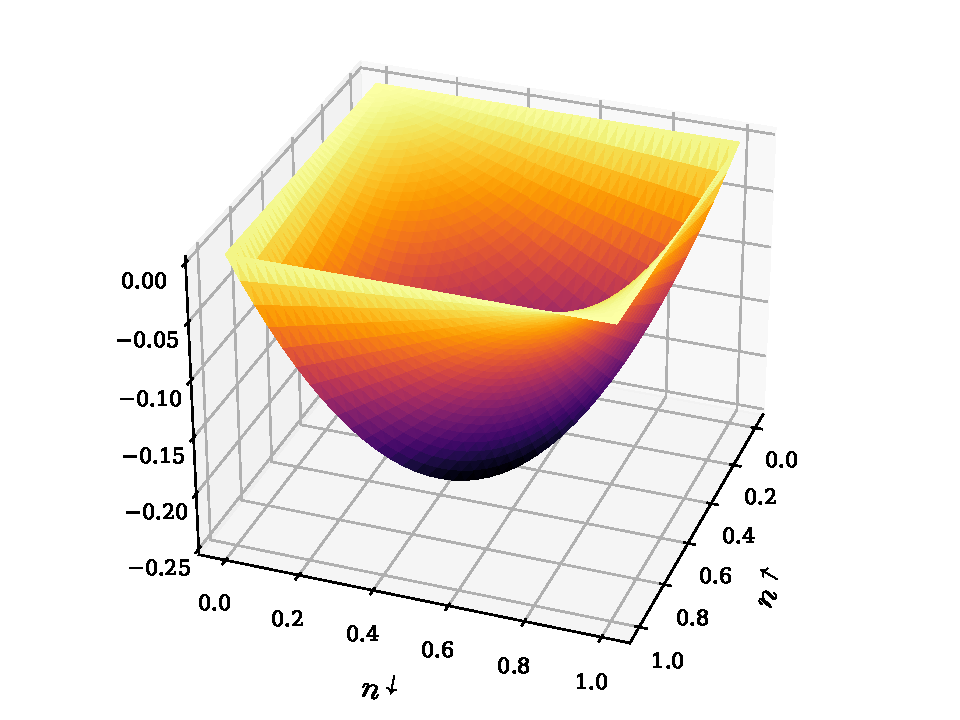
\includegraphics[width=0.5\columnwidth]{figures/novel_k_correction.pdf}
        \caption{My proposed second correction, $E_2(K, \{n^\sigma\})$ for addressing SCE, with $K = 1$}
        \label{fig:novel_k_correction}
    \end{figure}
\end{frame}
% %
\begin{frame}{Correction to SCE}
    \begin{columns}
        \column{0.38\linewidth}
        \centering
        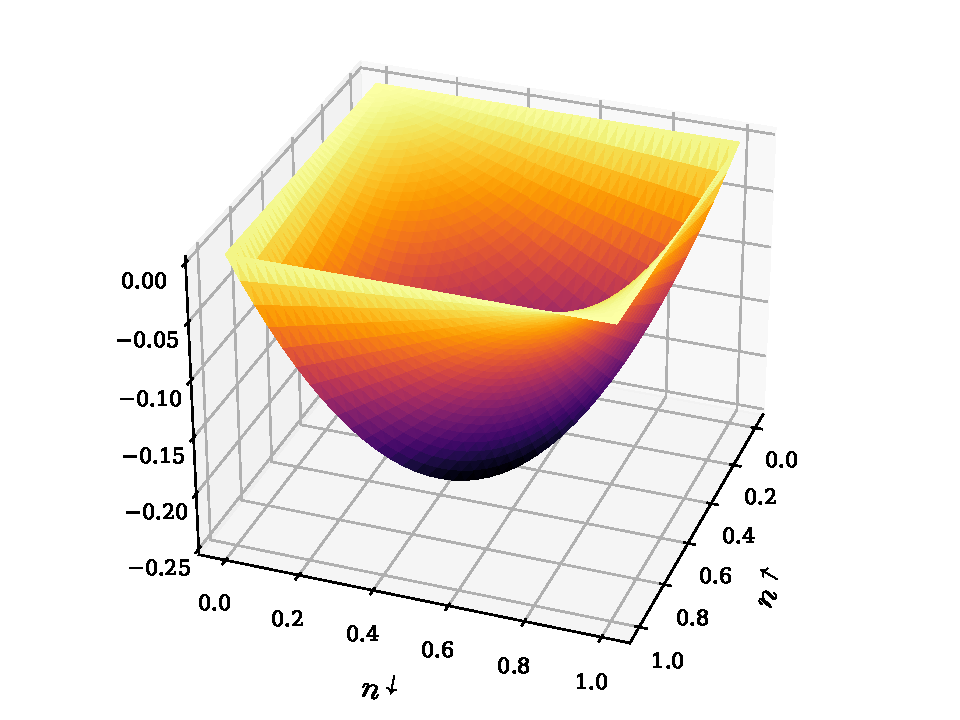
\includegraphics[width=1.2\columnwidth]{figures/novel_k_correction.pdf}
        \column{0.58\linewidth}
        \footnotesize
        This second energy correction term possesses the following important properties:
        %
        \begin{enumerate}
            \item it is zero for integer numbers of electrons (the four corners of \cref{fig:novel_k_correction})
            \item the curvature with respect to $\mu$ is controlled by the parameter $K$
                  \begin{equation}
                      \left.\frac{\partial^2 E_2}{\partial \mu^{2}}\right|_{n} = \frac{K}{2}
                  \end{equation}
            \item the curvature with respect to $n^\sigma$ is zero
                  \begin{equation}
                      \left.\frac{\partial^2 E_2}{\partial n^{\sigma 2}}\right|_{n^{-\sigma}} = 0
                  \end{equation}
        \end{enumerate}
        %
        However, by fulfilling these three properties it necessarily possesses one undesirable property: namely, the curvature with respect to the total occupancy $n = n^\uparrow + n^\downarrow$ is given by
        %
        \begin{equation}
            \left.\frac{\partial^2 E_2}{\partial n^{2}}\right|_{\mu} = -\frac{K}{2}
        \end{equation}
    \end{columns}
\end{frame}
% % %
% % which is unfortunately is non-zero. But as I argued earlier, perhaps this curvature is less important than those with respect to $n^\sigma$.
% % 
% % The resulting potential from this energy correction is given by $\hat v^\sigma_2[\rho] = v^\sigma_{2}(n_i^\uparrow, n_i^\downarrow) \ket{i}\bra{i}$ where
% % %
% % \begin{align}
% %     v^\sigma_2(n^\uparrow, n^\downarrow)
% %     = \frac{K}{2}\left[\frac{|\tilde n|}{\tilde n} + 1 - 2n^{-\sigma}\right]
% %     \label{eqn:novel_k_potential}
% % \end{align}
% % %
% % This is plotted in \cref{fig:novel_k_potential,fig:novel_k_potential_2d}.
% % 
% % It is important to note that despite the fact $E_2$ has no \emph{curvature} with respect to $n^\sigma$, the resulting potential does affect eigenvalues\footnote{More accurately, a $K$-correction will alter the eigenvalues of states with significant overlap with the Hubbard projector.} e.g.
% % %
% % \begin{equation}
% %     v^\sigma_2(n^\uparrow, n^\downarrow) = 
% %     \begin{cases}
% %         -n^{-\sigma} K     & \text{if } n < 1 \\
% %         (1 - n^{-\sigma})K & \text{if } n > 1
% %     \end{cases}
% % \end{equation}
% % %
% % We can interpret this linear correction as the correction to the eigenvalue required to guarantee the removal of SCE.
% % 
% % So now if we think of Fatemeh's CrI\textsubscript{3} example. Suppose $n_{mm}^\uparrow = 0.99$ and $n_{mm}^\downarrow = 0.0$. In this case $v_2^\uparrow = 0$ and $v_2^\downarrow = -0.99K$. $v_2^\sigma$ has very different behaviour either side of the $n = 1$ line, so for completeness consider the alternative case where $n_{mm}^\uparrow = 1.0$ and $n_{mm}^\downarrow = 0.01$. Qualitatively this is the same (one spin channel filled, the other empty) but it lies on the other side of the $n=1$ line. In this case $v_2^\uparrow = 0.99K$ and $v_2^\downarrow = 0$. So while the relative shift between the two levels is the same for these two cases, the absolute shift might lead to some pathologies.
% % %
% % \subsection{The combined correction}
% % \noindent Now let us consider the combined correction $E_1 + E_2$, and its effect on quasiparticle energies. From \cref{eqn:novel_u_potential,eqn:novel_k_potential} we have
% % %
\begin{frame}{The combined correction}
    \begin{figure}
        \centering
        \begin{subfigure}[b]{0.4\columnwidth}
            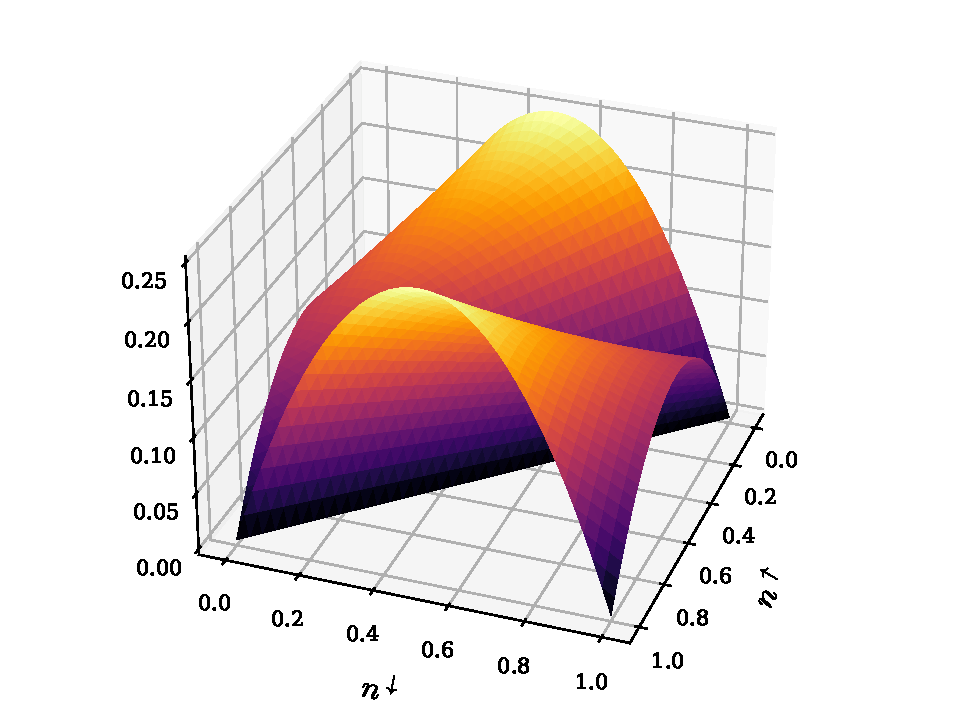
\includegraphics[width=\columnwidth]{figures/novel_u_correction.pdf}
            \caption{$E_1$ with $U^\uparrow = U^\downarrow/2$}
        \end{subfigure}
        \begin{subfigure}[b]{0.4\columnwidth}
            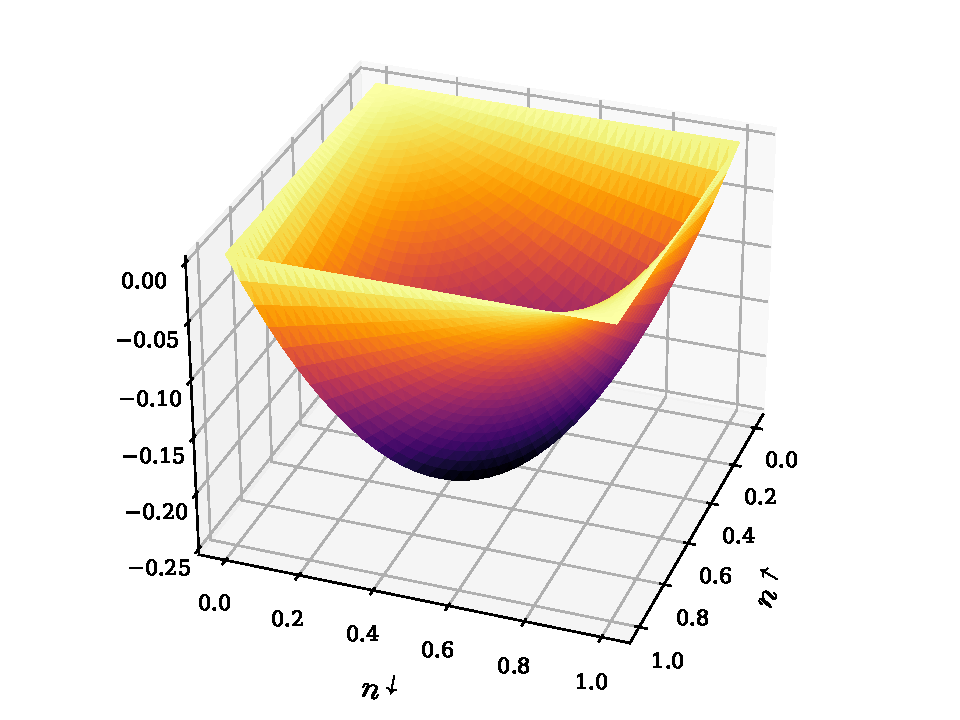
\includegraphics[width=\columnwidth]{figures/novel_k_correction.pdf}
            \caption{$E_2$}
        \end{subfigure}
    \end{figure}
    \begin{equation}
        v^\sigma(n^\uparrow, n^\downarrow) =
        \begin{cases}
            {U^\sigma}
            \left(\frac{1}{2} - n^\sigma\right)
            +
            \left(
            1 - n^{-\sigma}
            \right)
            \left(
            \frac{U^\uparrow + U^\downarrow}{2}
            +K
            \right)
             & n > 1 \\
            U^\sigma
            \left(
            \frac{1}{2}
            -n^{\sigma}
            \right)
            - n^{-\sigma}
            \left(
            \frac{U^\uparrow + U^\downarrow}{2}
            + K
            \right)
             & n < 1
        \end{cases}
        \label{eqn:the_combined_potential}
    \end{equation}
\end{frame}
% %
% \Cref{eqn:the_combined_potential} is one of the main results of this work. The first term is the familiar conventional +\emph{U} potential with a spin-dependent $U$. The second term is less familiar. It introduces a $n^{-\sigma}$-dependent shift with a discontinuity across $n = 1$ of magnitude
% %
% \begin{equation}
% \lim_{n\rightarrow 1^+} v^\sigma
% - \lim_{n\rightarrow 1^-} v^\sigma
% = 
%     \frac{U^\uparrow + U^\downarrow}{2}
%     + K
% \end{equation}
% %
% I need to think more to understand this discontinuity and its origins. Additionally, the particular combination of the parameters $\frac{U^\uparrow + U^\downarrow}{2} + K$ is important. Note that if we set $K = -\frac{U^\uparrow + U^\downarrow}{2}$ we return to conventional DFT\,+\,\emph{U}. (This corresponds to deploying the $K$-correction to add back in the curvature with respect to $\mu$ that the conventional $+U$ correction erroneously includes but my $+U$ correction correctly does not possess.)
% 
% I worry that this discontinuity will lead to strange behaviour and thereby render my correction unusable. 
% 
% \section{Determining $U^\sigma$ and $K$ via linear response}
\begin{frame}{Determining $U^\sigma$ and $K$ via spin-resolved LR}
    % For these functionals, we want to be able to appropriately determine $U^\uparrow$, $U^\downarrow$, and $K$ via linear response, from the spin-resolved response matrices $\chi_{II}^{\sigma\sigma'}$ and $(\chi_0)_{II}^{\sigma\sigma'}$ and the resulting quantity
    % %
    % \begin{equation}
    %     f^{\sigma\sigma'}_{II} = \left((\chi_{0II})^{-1} - (\chi_{II})^{-1}\right)^{\sigma\sigma'}
    % \end{equation}
    % %
    % where note that we are inverting separately the block matrices $\chi_{II}$ rather than inverting the entire matrix $\chi$ and then focusing on the block corresponding to Hubbard site $I$. Because in this way we have entirely decoupled Hubbard sites, I will from now on drop the Hubbard site indices.
    % 
    % In order to relate the parameters $U^\sigma$ and $K$ to the elements of $f^{\sigma \sigma'}$ it is necessary to compute some derivatives. These are computed in \cref{sec:derivatives}; to summarise the results of that appendix
    % %
    \begin{equation}
        \left.\frac{\partial ^2}{\partial n^{\sigma 2}} \left(E_1 + E_2\right) \right|_{n^{-\sigma}} = -U^\sigma
    \end{equation}
    %
    and thus it follows that we should set $U^\sigma = U^{\sigma\sigma}$. Meanwhile, the mixed derivatives
    %
    \begin{align}
        \left.\frac{\partial }{\partial n^{\sigma}}\left[\left.\frac{\partial }{\partial n^{-\sigma}} \left(E_1 + E_2\right) \right|_{n^{\sigma}}\right]\right|_{n^{-\sigma}}
        = -\frac{U^\uparrow + U^\downarrow + K}{2}
    \end{align}
    %
    and thus by equating the LHS with $-\frac{1}{2}(U^{\uparrow\downarrow} + U^{\downarrow \uparrow})$ it follows that $K = - U^{\uparrow\uparrow} + U^{\uparrow\downarrow} + U^{\downarrow\uparrow} - U^{\downarrow\downarrow}$
\end{frame}
% % 
% % Note to self: might be out by a factor of 2 here and there...
% % 
% % \section{Generalisation to multi-orbital Hubbard subspaces}
% % Thus far I have only presented corrections that can be applied to a \emph{1s} Hubbard subspace. In order for these corrections to be generally applicable, they must be generalised to multi-orbital Hubbard subspaces.
% % 
% % The approach for this generalisation would be to look for a matrix representation of our corrections that, in the basis of functions that diagonalise $n$, reduce down to applying the corrections \cref{eqn:novel_u_correction,eqn:novel_k_correction} to the eigenvalues of $n$.
% % 
% % In conventional DFT\,+\,\emph{U} this is straightforward: we have a one-site correction like $\sum_{i\sigma} \lambda^\sigma_i(1 - \lambda^\sigma_i) = \sum_{i\sigma} \trace{\mathbf{n}^\sigma(1 - \mathbf{n}^\sigma)}$ where we have taken advantage of the fact that the trace of a matrix is invariant under basis transformations to obtain a rotationally-invariant formulation.
% % 
% % However, my novel corrections include terms like $\sum_i |\lambda^\sigma_i + \lambda^\sigma_i - 1|$. These terms cannot be reduced to matrix traces. Therefore in order to evaluate them we must explicitly diagonalise $\mathbf{n}$.
% % 
% % \section{Application to C\lowercase{r}I\textsubscript{3} (WIP)}
% \begin{frame}{Application to C\lowercase{r}I\textsubscript{3} (WIP)}
%     % For CrI\textsubscript{3}, we performed spin-polarised DFPT calculations, and obtained the following response matrices:
%     % %
%     % \begin{align}
%     %     \chi^{\sigma\sigma'} = 
%     %     \begin{pmatrix}
%     %     -0.192107 & 0.140612 \\
%     %     0.140612 & -0.213558
%     %     \end{pmatrix};
%     %     \qquad
%     %     \chi_0^{\sigma\sigma'} = 
%     %     \begin{pmatrix}
%     %     -0.285342 & 0.0 \\
%     %     0.0 & -0.225989
%     %     \end{pmatrix}
%     % \end{align}
%     % %
%     % It follows that
%     % %
%     % \begin{align}
%     %     f^{\sigma\sigma'}
%     %     = \left(\chi_0^{-1} - \chi^{-1}\right)_{\sigma\sigma'}
%     %     =
%     %     \begin{pmatrix}
%     %         6.54321121 & 6.61571148 \\
%     %         6.61571148 & 4.61352665
%     %     \end{pmatrix}
%     %     _{\sigma\sigma'}
%     % \end{align}
%     % %
%     % from which we can extract the parameters $U^\uparrow = 6.54$ eV, $U^\downarrow = 4.61$ eV, and $K = 2.07$ eV.
%     $U^\uparrow = 6.54$ eV, $U^\downarrow = 4.61$ eV, and $K = 2.07$ eV.
% 
%     At the PBE level, the eigenvalues of $\mathbf{n}^\sigma$ are given by three orbitals with spin-resolved occupancy $(0.971, 0.065)$ and two with occupancy $(0.472, 0.245)$. Suppose we have a KS state that lies entirely in the subspace spanned by the three degenerate orbitals. Then
%     %
%     \begin{equation}
%         v^\sigma(0.971, 0.065) =
%         U^\sigma
%         \left(
%         \frac{1}{2}
%         -n^{\sigma}
%         \right)
%         +
%         \left(
%         1
%         - n^{-\sigma}
%         \right)
%         \left(
%         \frac{U^\uparrow + U^\downarrow}{2}
%         +K
%         \right)
%         =
%         \begin{cases}
%             4.07 & \sigma = \uparrow   \\
%             2.23 & \sigma = \downarrow
%         \end{cases}
%     \end{equation}
%     %
%     % This appears strange; in the typical picture we expect the potential for a filled orbital to be negative and an empty orbital, positive. Clearly this discontinuity is dominating the correction (which is unsurprising, given that its prefactor will likely be larger than $U^\sigma$).
% 
%     Meanwhile, suppose we have a KS state that lies entirely in the subspace spanned by the two other orbitals. Then
%     %
%     \begin{equation}
%         v^\sigma(0.472, 0.245) =
%         U^\sigma
%         \left(
%         \frac{1}{2}
%         -n^{\sigma}
%         \right)
%         - n^{-\sigma}
%         \left(
%         \frac{U^\uparrow + U^\downarrow}{2}
%         + K
%         \right)
%         =
%         \begin{cases}
%             -1.69 & \sigma = \uparrow   \\
%             -2.44 & \sigma = \downarrow
%         \end{cases}
%     \end{equation}
% \end{frame}
% %
% Ignoring any screening, these are the amounts by which these orbitals would be shifted in energy. If this correction is going to be any good at all, the screening effects would have to be considerable!
% 
% \section{Conclusions}
% \cref{eqn:novel_u_correction,eqn:novel_k_correction} are promising corrections to DFT that separately address self interaction error and static correlation without coupling the two. They are also non-zero at integer occpuancies. This means that they possess several key properties that state-of-the-art DFT\,+\,\emph{U}\,+\,\emph{J} lacks. I still need to work out how to generalise these corrections to multi-orbital Hubbard parameters. If we can do this, then all that remains is to implement them in \textsc{Quantum} ESPRESSO. Only then will we be able to determine if the numerics of these functionals is sufficiently well-behaved, and if they ultimately yield good results.
% 
% It is important to acknowledge that Kulik and co-workers experimented with a very similar functional to the ones I have presented in this work (Ref \cite{Bajaj2017}). Their formulation was a little less elegant than mine (if I may say so) because their correction was parametrised by 8 parameters (rather than my three $U^\uparrow$, $U^\downarrow$, and $K$). The reason why I was able to use far fewer parameters is because my functional imposes several key properties explicitly e.g. my functional corrections are continuous across the line $n = 1$. In contrast, their their functional would only be continuous across $n = 1$ for very particular combinations of their 8 parameters. Ultimately they abandoned their model, saying that ``the large number and non-intuitive nature of these parameters, including linear terms and constants, leads us to disfavor this correction form''. In contrast, I have shown that corrections of this form only require a few parameters and these parameters are concretely related to specific curvatures of the system. I therefore draw the opposite conclusion to them: I believe that these corrections are promising and warrant further investigation.
% 
% \appendix
% \section{Derivatives of $E_1$ and $E_2$}
% \label{sec:derivatives}
% \subsection{First order derivatives}
% \noindent The derivative of $E_1$ with respect to $n_\sigma$ is
% %
% \begin{align}
%     \left.\frac{\partial E_1}{\partial n^{\sigma}} \right|_{n^{-\sigma}}
%     = & 
%     \sum_{\sigma'} \frac{U^{\sigma'}}{4} \left.\frac{\partial}{\partial n^{\sigma}}\left[|\tilde n| + \tilde n(1 - 2n^{\sigma'})\right] \right|_{n^{-\sigma}}
%     =
%     \sum_{\sigma'} \frac{U^{\sigma'}}{4} \left[\frac{|\tilde n|}{\tilde n} + 1 - 2(n^{\sigma'} + \delta_{\sigma\sigma'}\tilde n)\right]
% \end{align}
% %
% and
% %
% \begin{align}
%     \left.\frac{\partial E_2}{\partial n^{\sigma}} \right|_{n^{-\sigma}}
%     = & 
%     \frac{K}{4}\left.\frac{\partial}{\partial n^{\sigma}}\left[(n^\uparrow-n^\downarrow)^2-(|\tilde n|-1)^2\right] \right|_{n^{-\sigma}}
%     =
%     \frac{K}{2}\left[n^\sigma-n^{-\sigma}-\tilde n+\frac{|\tilde n|}{\tilde n}\right]
% \end{align}
% %
% \subsection{Second order derivatives}
% \noindent Now to calculate the second derivatives:
% %
% \begin{equation}
%     \left.\frac{\partial^2 E_1}{\partial n^{\sigma 2}} \right|_{n^{-\sigma}}
%     = 
%     \sum_{\sigma'} \frac{U^{\sigma'}}{4} \left.\frac{\partial}{\partial n^{\sigma}}\left[\frac{|\tilde n|}{\tilde n} + 1 - 2(n^{\sigma'} + \delta_{\sigma\sigma'}\tilde n)\right] \right|_{n^{-\sigma}}
%     = -U^\sigma
% \end{equation}
% %
% and
% %
% \begin{align}
%     \left.\frac{\partial}{\partial n^{-\sigma}}\left(\left.\frac{\partial E_1}{\partial n^{\sigma}}\right|_{n^{-\sigma}}\right) \right|_{n^{\sigma}}
%     = &
%     \sum_{\sigma'} \frac{U^{\sigma'}}{4} \left.\frac{\partial}{\partial n^{-\sigma}}\left[\frac{|\tilde n|}{\tilde n} + 1 - 2(n^{\sigma'} + \delta_{\sigma\sigma'}\tilde n)\right] \right|_{n^{\sigma}}
%     \nonumber \\
%     = & 
%     -\frac{1}{2}\left.\frac{\partial}{\partial n^{-\sigma}}\left[U^{\sigma}\tilde n + \sum_{\sigma'}U^{\sigma'} n^{\sigma'} \right] \right|_{n^{\sigma}}
%     \nonumber \\
%     = & 
%     -\frac{U^\uparrow + U^\downarrow}{2}
% \end{align}
% %
% and
% %
% \begin{equation}
%     \left.\frac{\partial^2 E_2}{\partial n^{\sigma 2}} \right|_{n^{-\sigma}}
%     = 
%     \frac{K}{2}\left.\frac{\partial}{\partial n^{\sigma}}
%     \left[n^\sigma-n^{-\sigma}-\tilde n+\frac{|\tilde n|}{\tilde n}\right]
%     \right|_{n^{-\sigma}}
%     = 0
% \end{equation}
% %
% and
% %
% \begin{align}
%     \left.\frac{\partial}{\partial n^{-\sigma}}\left(\left.\frac{\partial E_2}{\partial n^{\sigma}}\right|_{n^{-\sigma}}\right) \right|_{n^{\sigma}}
%     = &
%     \frac{K}{2}\left.\frac{\partial}{\partial n^{-\sigma}}
%     \left[n^\sigma-n^{-\sigma}-\tilde n+\frac{|\tilde n|}{\tilde n}\right]
%     \right|_{n^{\sigma}}
%     = 
%     -\frac{K}{2}
% \end{align}
%

\begin{frame}{Rethinking inter-spin corrections}
    My new functional
    \footnotesize
    \begin{columns}
        \column{0.3\linewidth}
        \begin{figure}
            \centering
            \begin{subfigure}[b]{\columnwidth}
                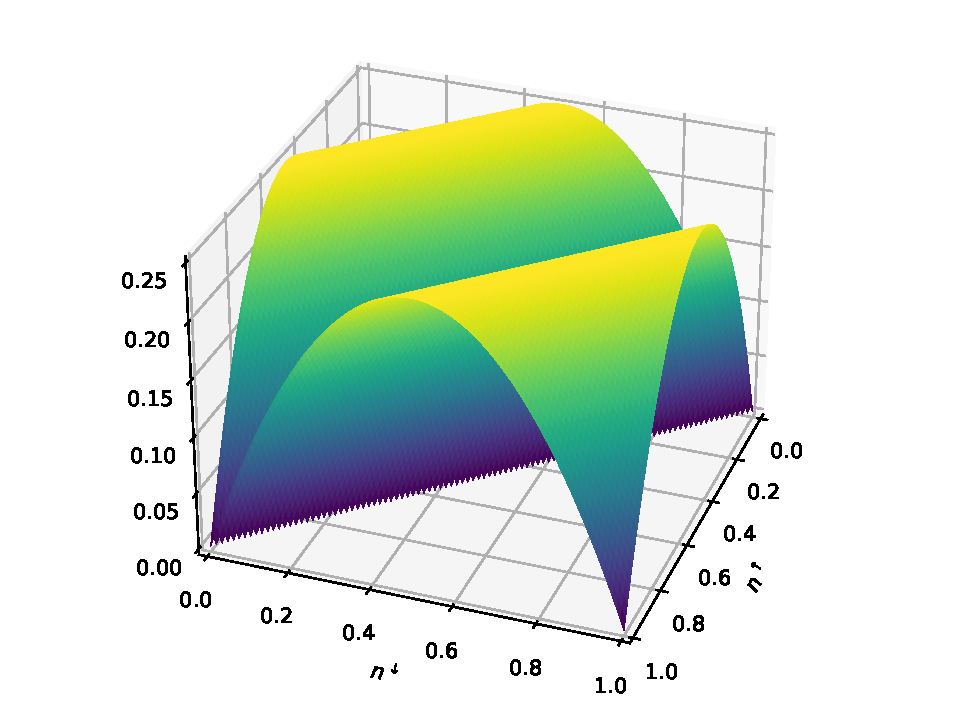
\includegraphics[width=\columnwidth]{figures/novel_u_correction_equal.pdf}
            \end{subfigure}
            \begin{subfigure}[b]{\columnwidth}
                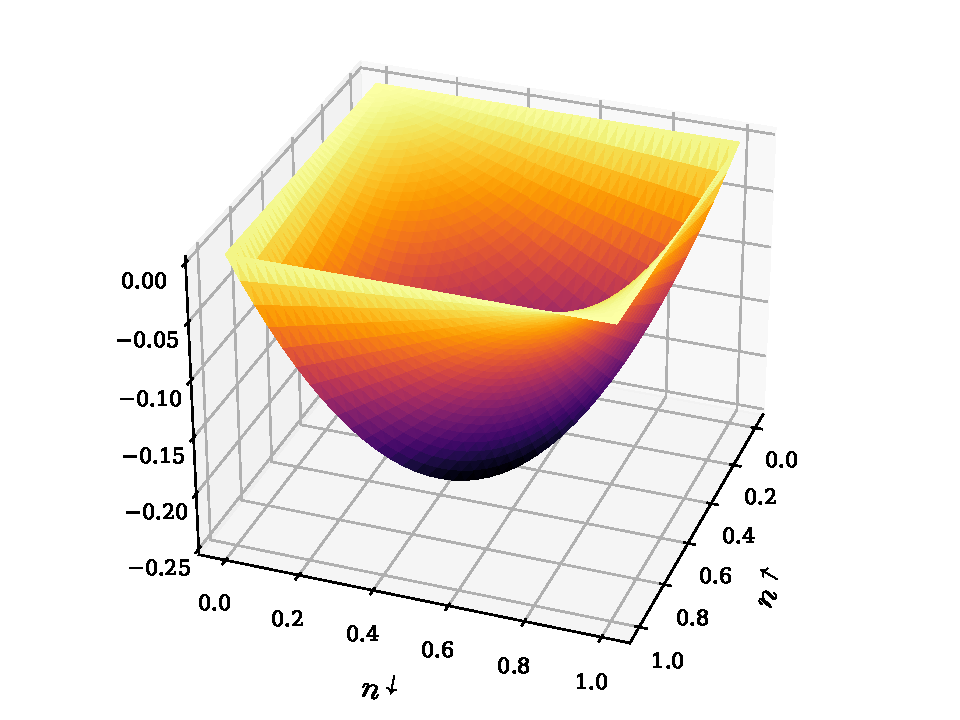
\includegraphics[width=\columnwidth]{figures/novel_k_correction.pdf}
            \end{subfigure}
        \end{figure}
        \column{0.68\linewidth}
        \begin{equation}
            E_1(\{U^\sigma\}, \{n^\sigma\}) =
            \sum_\sigma \frac{U^\sigma}{2} \left(n^\uparrow + n^\downarrow - 1\right) \times
            \begin{cases}
                -n^\sigma    & n < 1 \\
                1 - n^\sigma & n > 1
            \end{cases}
        \end{equation}
        \begin{equation}
            E_2(K, \{n^\sigma\}) % = & \frac{K}{4}\left[(n^\uparrow-n^\downarrow)^2-(|\tilde n|-1)^2\right] \nonumber \\
            % = & \frac{K}{4}\left[(n^\uparrow)^2 - 2n^\uparrow n^\downarrow + (n^\downarrow)^2-(n^\uparrow + n^\downarrow - 1)^2 + 2(|n^\uparrow + n^\downarrow - 1|) -1)\right] \nonumber \\
            % = & \frac{K}{2}\left[- 2 n^\uparrow n^\downarrow + n^\uparrow + n^\downarrow - 1 + (|n^\uparrow + n^\downarrow - 1|)\right] \nonumber \\
            = \begin{cases}
                - Kn^\uparrow n^\downarrow            & n < 1 \\
                - K(1 - n^\uparrow)(1 - n^\downarrow) & n > 1
            \end{cases}
        \end{equation}

        \begin{equation}
            v^\sigma(n^\uparrow, n^\downarrow) =
            \begin{cases}
                {U^\sigma}
                \left(\frac{1}{2} - n^\sigma\right)
                +
                \left(
                1 - n^{-\sigma}
                \right)
                \left(
                \frac{U^\uparrow + U^\downarrow}{2}
                +K
                \right)
                 & n > 1 \\
                U^\sigma
                \left(
                \frac{1}{2}
                -n^{\sigma}
                \right)
                - n^{-\sigma}
                \left(
                \frac{U^\uparrow + U^\downarrow}{2}
                + K
                \right)
                 & n < 1
            \end{cases}
            \label{eqn:the_combined_potential}
        \end{equation}
        Open questions:
        \begin{itemize}
            \item does this fix total energies?
            \item is the discontinuity at $n=1$ a problem?
            \item how best to generalise to multiple orbitals?
            \item what is the effect of orbital relaxation?
        \end{itemize}
    \end{columns}
\end{frame}

\begin{frame}{Linearization}

\end{frame}

\begin{frame}{DFT+U}

\end{frame}

\begin{frame}{Acknowledgements}

   \begin{center}
      \footnotesize
      \begin{tabularx}{0.5\textwidth}{CC}
         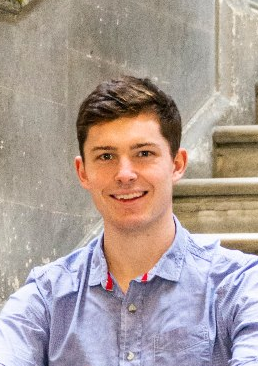
\includegraphics[height = 0.4\paperheight]{photos/andrew_burgess.png}     &
         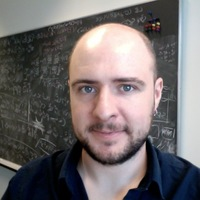
\includegraphics[height = 0.4\paperheight]{figures/david_oregan.jpg}    \\
         % 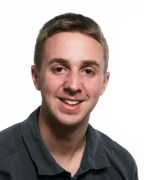
\includegraphics[height = 0.2\paperheight]{figures/daniel_cole.jpeg}       &
         % 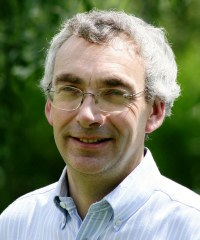
\includegraphics[height = 0.2\paperheight]{figures/mike_payne.jpeg}        &
         % 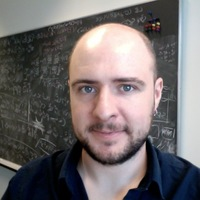
\includegraphics[height = 0.2\paperheight]{figures/david_oregan.jpg}         \\
         Andrew Burgess                                                             &
         David O'Regan                                                             \\
      \end{tabularx}
   \end{center}

   \vspace{1ex}
   \begin{center}
      paper available at PRB 107, L121115 (2023) | slides available at 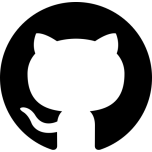
\includegraphics[height=\fontcharht\font`\B]{logos/github-favicon.png} github/elinscott
   \end{center}


   % \begin{multicols}{2}
   %    \tiny
   %    \printbibliography
   %    \normalsize
   % \end{multicols}
   \vspace{2ex}
   \scriptsize

   \setbeamercolor*{bibliography entry title}{fg=black}
   \setbeamercolor*{bibliography entry author}{fg=black}
   \setbeamercolor*{bibliography entry location}{fg=black}
   \setbeamercolor*{bibliography entry note}{fg=black}

   \vspace{2ex}
   \scriptsize
\end{frame}

\backupbegin
\begin{frame}{}

   \begin{center}
      \huge SPARE SLIDES
   \end{center}

\end{frame}

\begin{frame}{Spare slide}
\end{frame}


% \begin{frame}{References}
%    \setbeamercolor*{bibliography entry title}{fg=black}
%    \setbeamercolor*{bibliography entry author}{fg=black}
%    \setbeamercolor*{bibliography entry location}{fg=black}
%    \setbeamercolor*{bibliography entry note}{fg=black}
%    \printbibliography
%    % For further reading on Koopmans functionals, see \cite{Dabo2010,Borghi2014,Nguyen2018,Colonna2018,Colonna2019,DeGennaro2022,Colonna2022}
% 
% \end{frame}
% \begin{frame}{Learning the screening parameters}
%    \begin{center}
%       \begin{tikzpicture}
%          \node[inner sep=0pt] (water box) at (0,0)
%          {
%             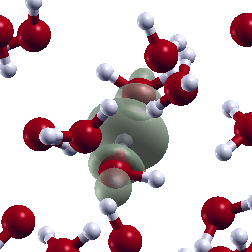
\includegraphics[width=0.25\textwidth]{figures/orbital.emp.00191_cropped.png}
%          };
%          \node[below=0cm of water box] (density) {$\rho_i(\mathbf{r})$};
%          \node[right=0.2\textwidth of water box] (power spectrum) {
%             $
%                \begin{bmatrix}
%                   x_{0} \\
%                   x_{1} \\
%                   x_{2} \\
%                   \vdots
%                \end{bmatrix}
%             $
%          };
%          \path[line] (water box) -- node [midway, above, align=center] (decomposition) {power spectrum \\ decomposition} (power spectrum);
%          \node[right=0.2\textwidth of power spectrum] (screening parameter) {$\alpha_i$};
%          \path[line] (power spectrum) -- node [midway, above, align=center] (model) {ML model} (screening parameter);
%       \end{tikzpicture}
%    \end{center}
% 
%    \vspace{-4em}
% 
%    \blfootcite{Schubert2022}
% 
%    \begin{align*}
%       c^i_{nlm,k=\mathsf{orbital}} & =\int d\textbf{r} g_{nl}(r)Y_{lm}(\theta,\varphi)\rho^i(\textbf{r}-\textbf{R}^i)                        \\
%       p^i_{n_1n_2l,k_1k_2}         & =\pi \sqrt{\frac{8}{2l+1}}\sum\limits_m {c_{n_1lm,k_1}^{i *}}c_{n_2lm,k_2}^i \label{eq: power spectrum}
%    \end{align*}
% 
%    % $g_{nl}$ = orthonormalised radial Gaussian basis functions
% 
%    % $Y_{lm}$ = spherical harmonics
% 
% \end{frame}
% 
% \begin{frame}{Learning the screening parameters}
%    \begin{center}
% 
%       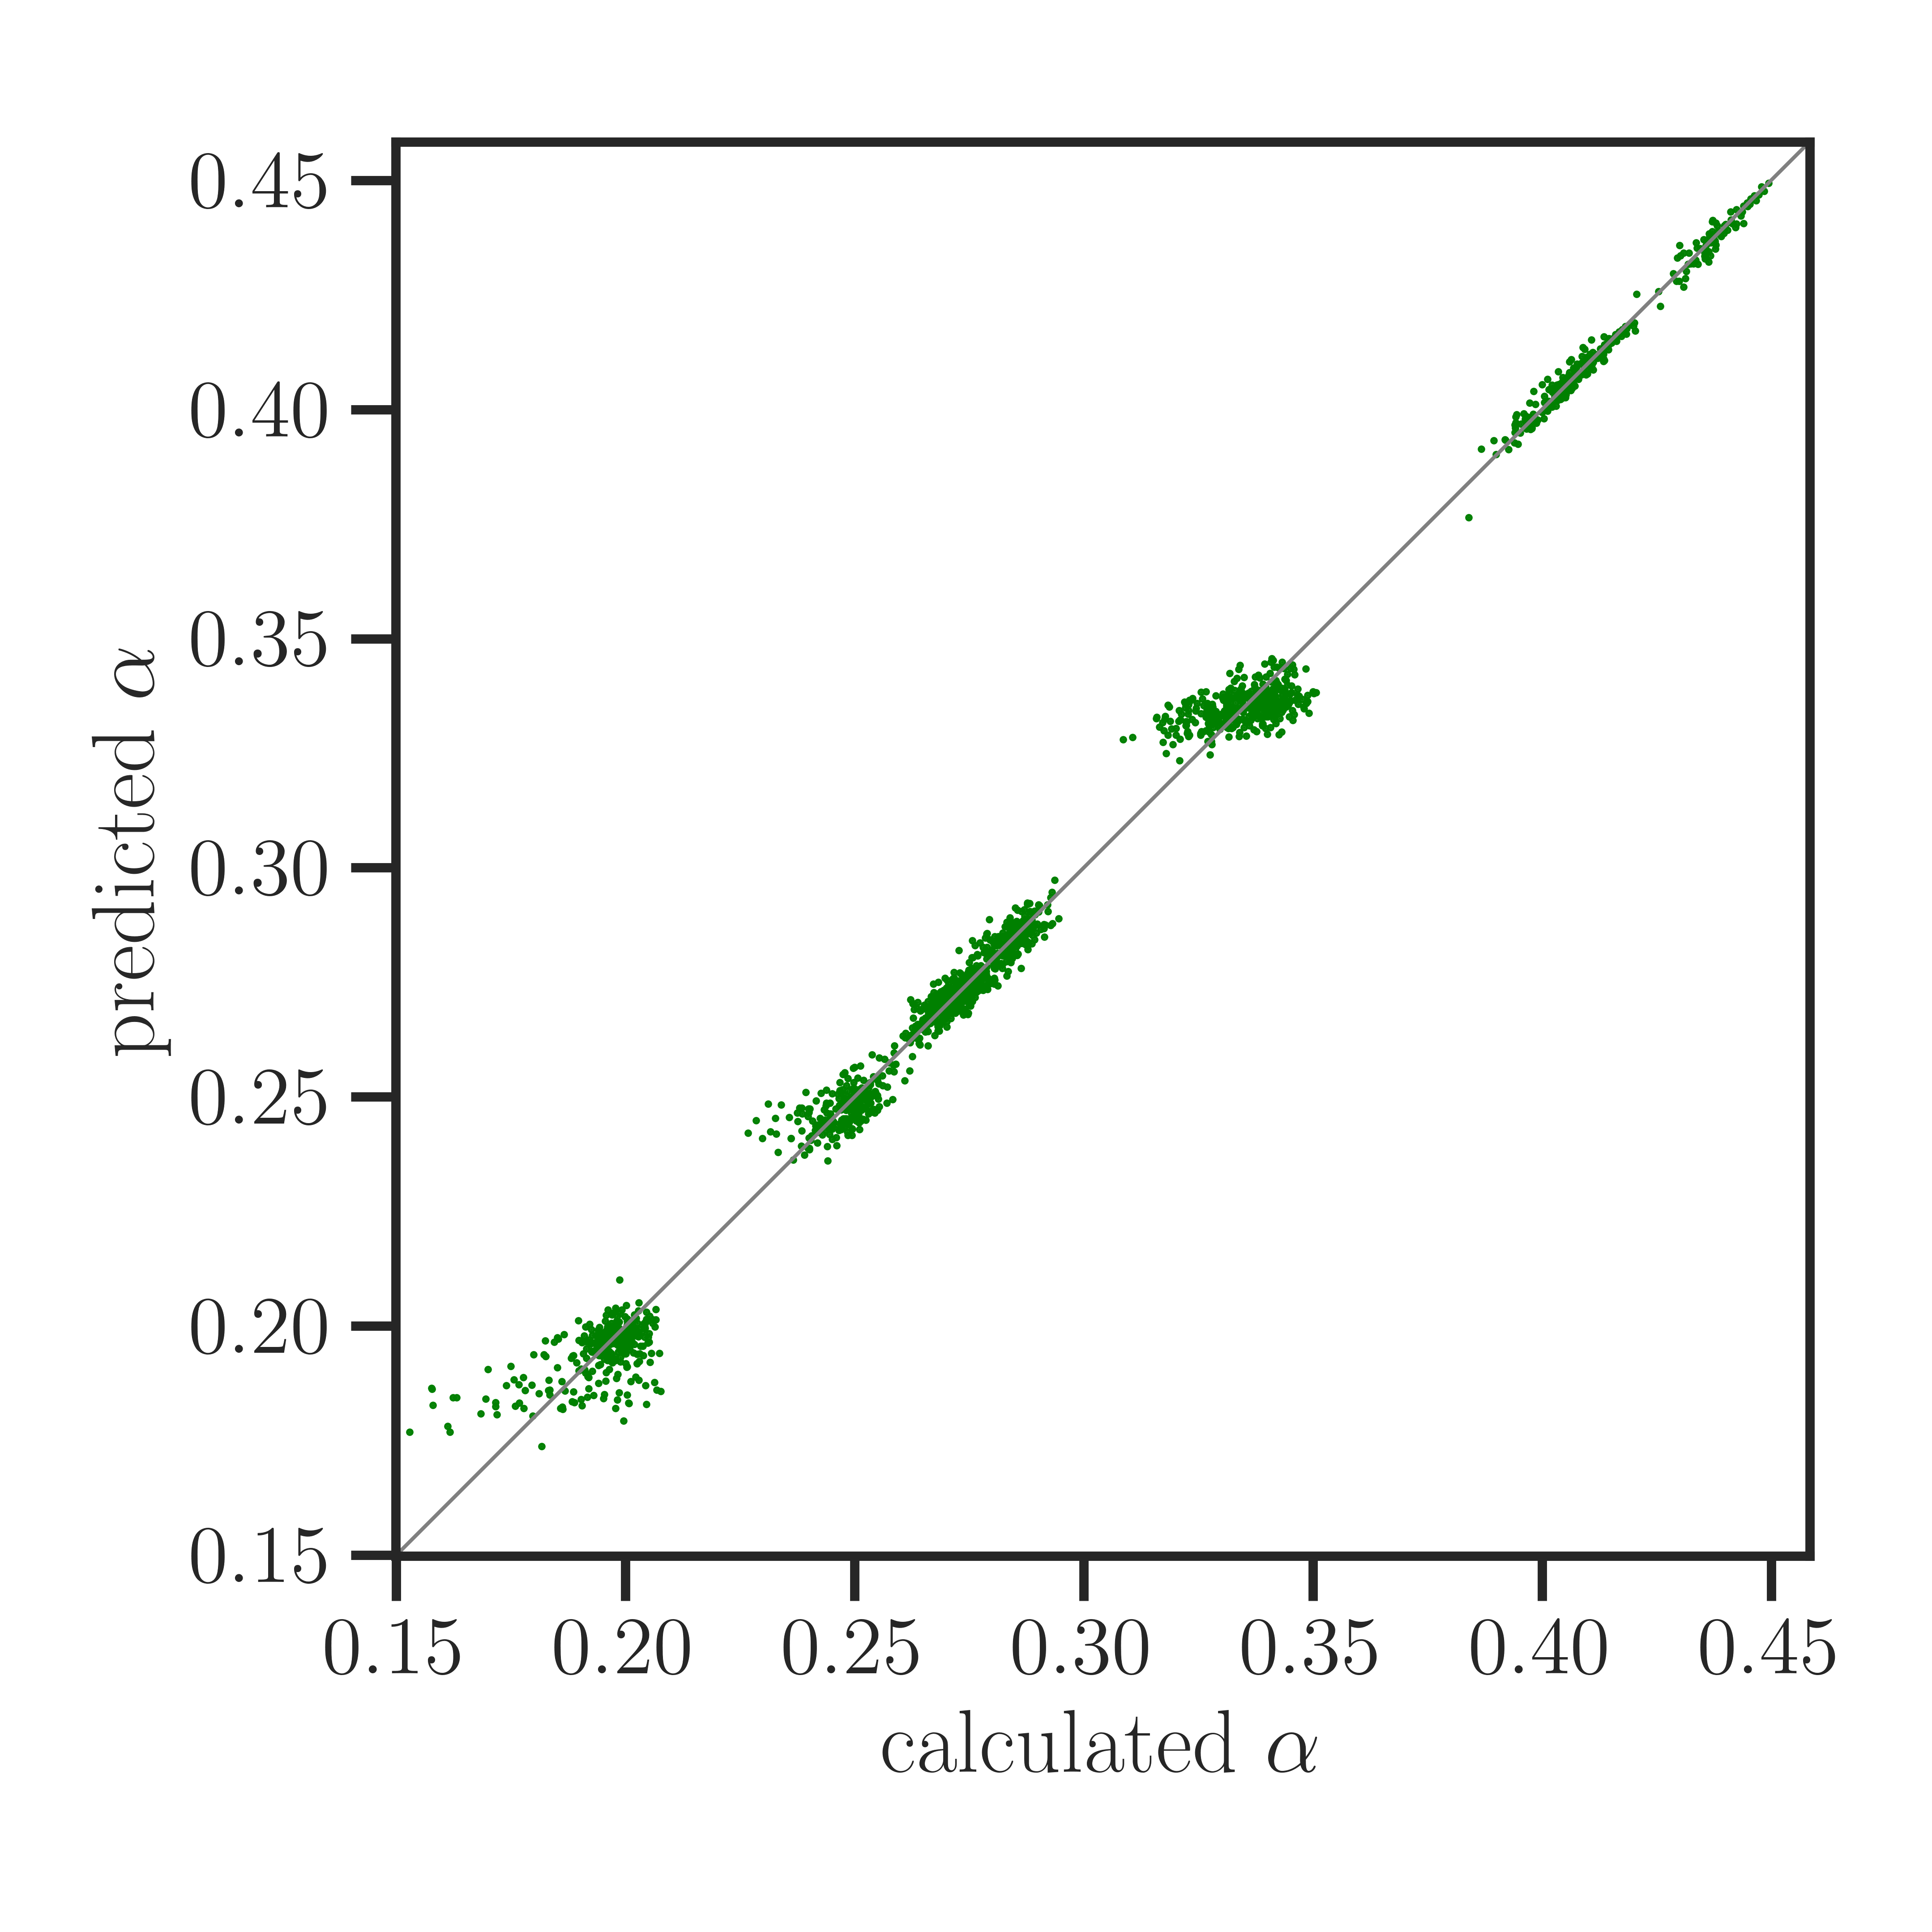
\includegraphics[height=0.7\paperheight]{figures/CsSnI3_calc_vs_pred_Edward.png}
%       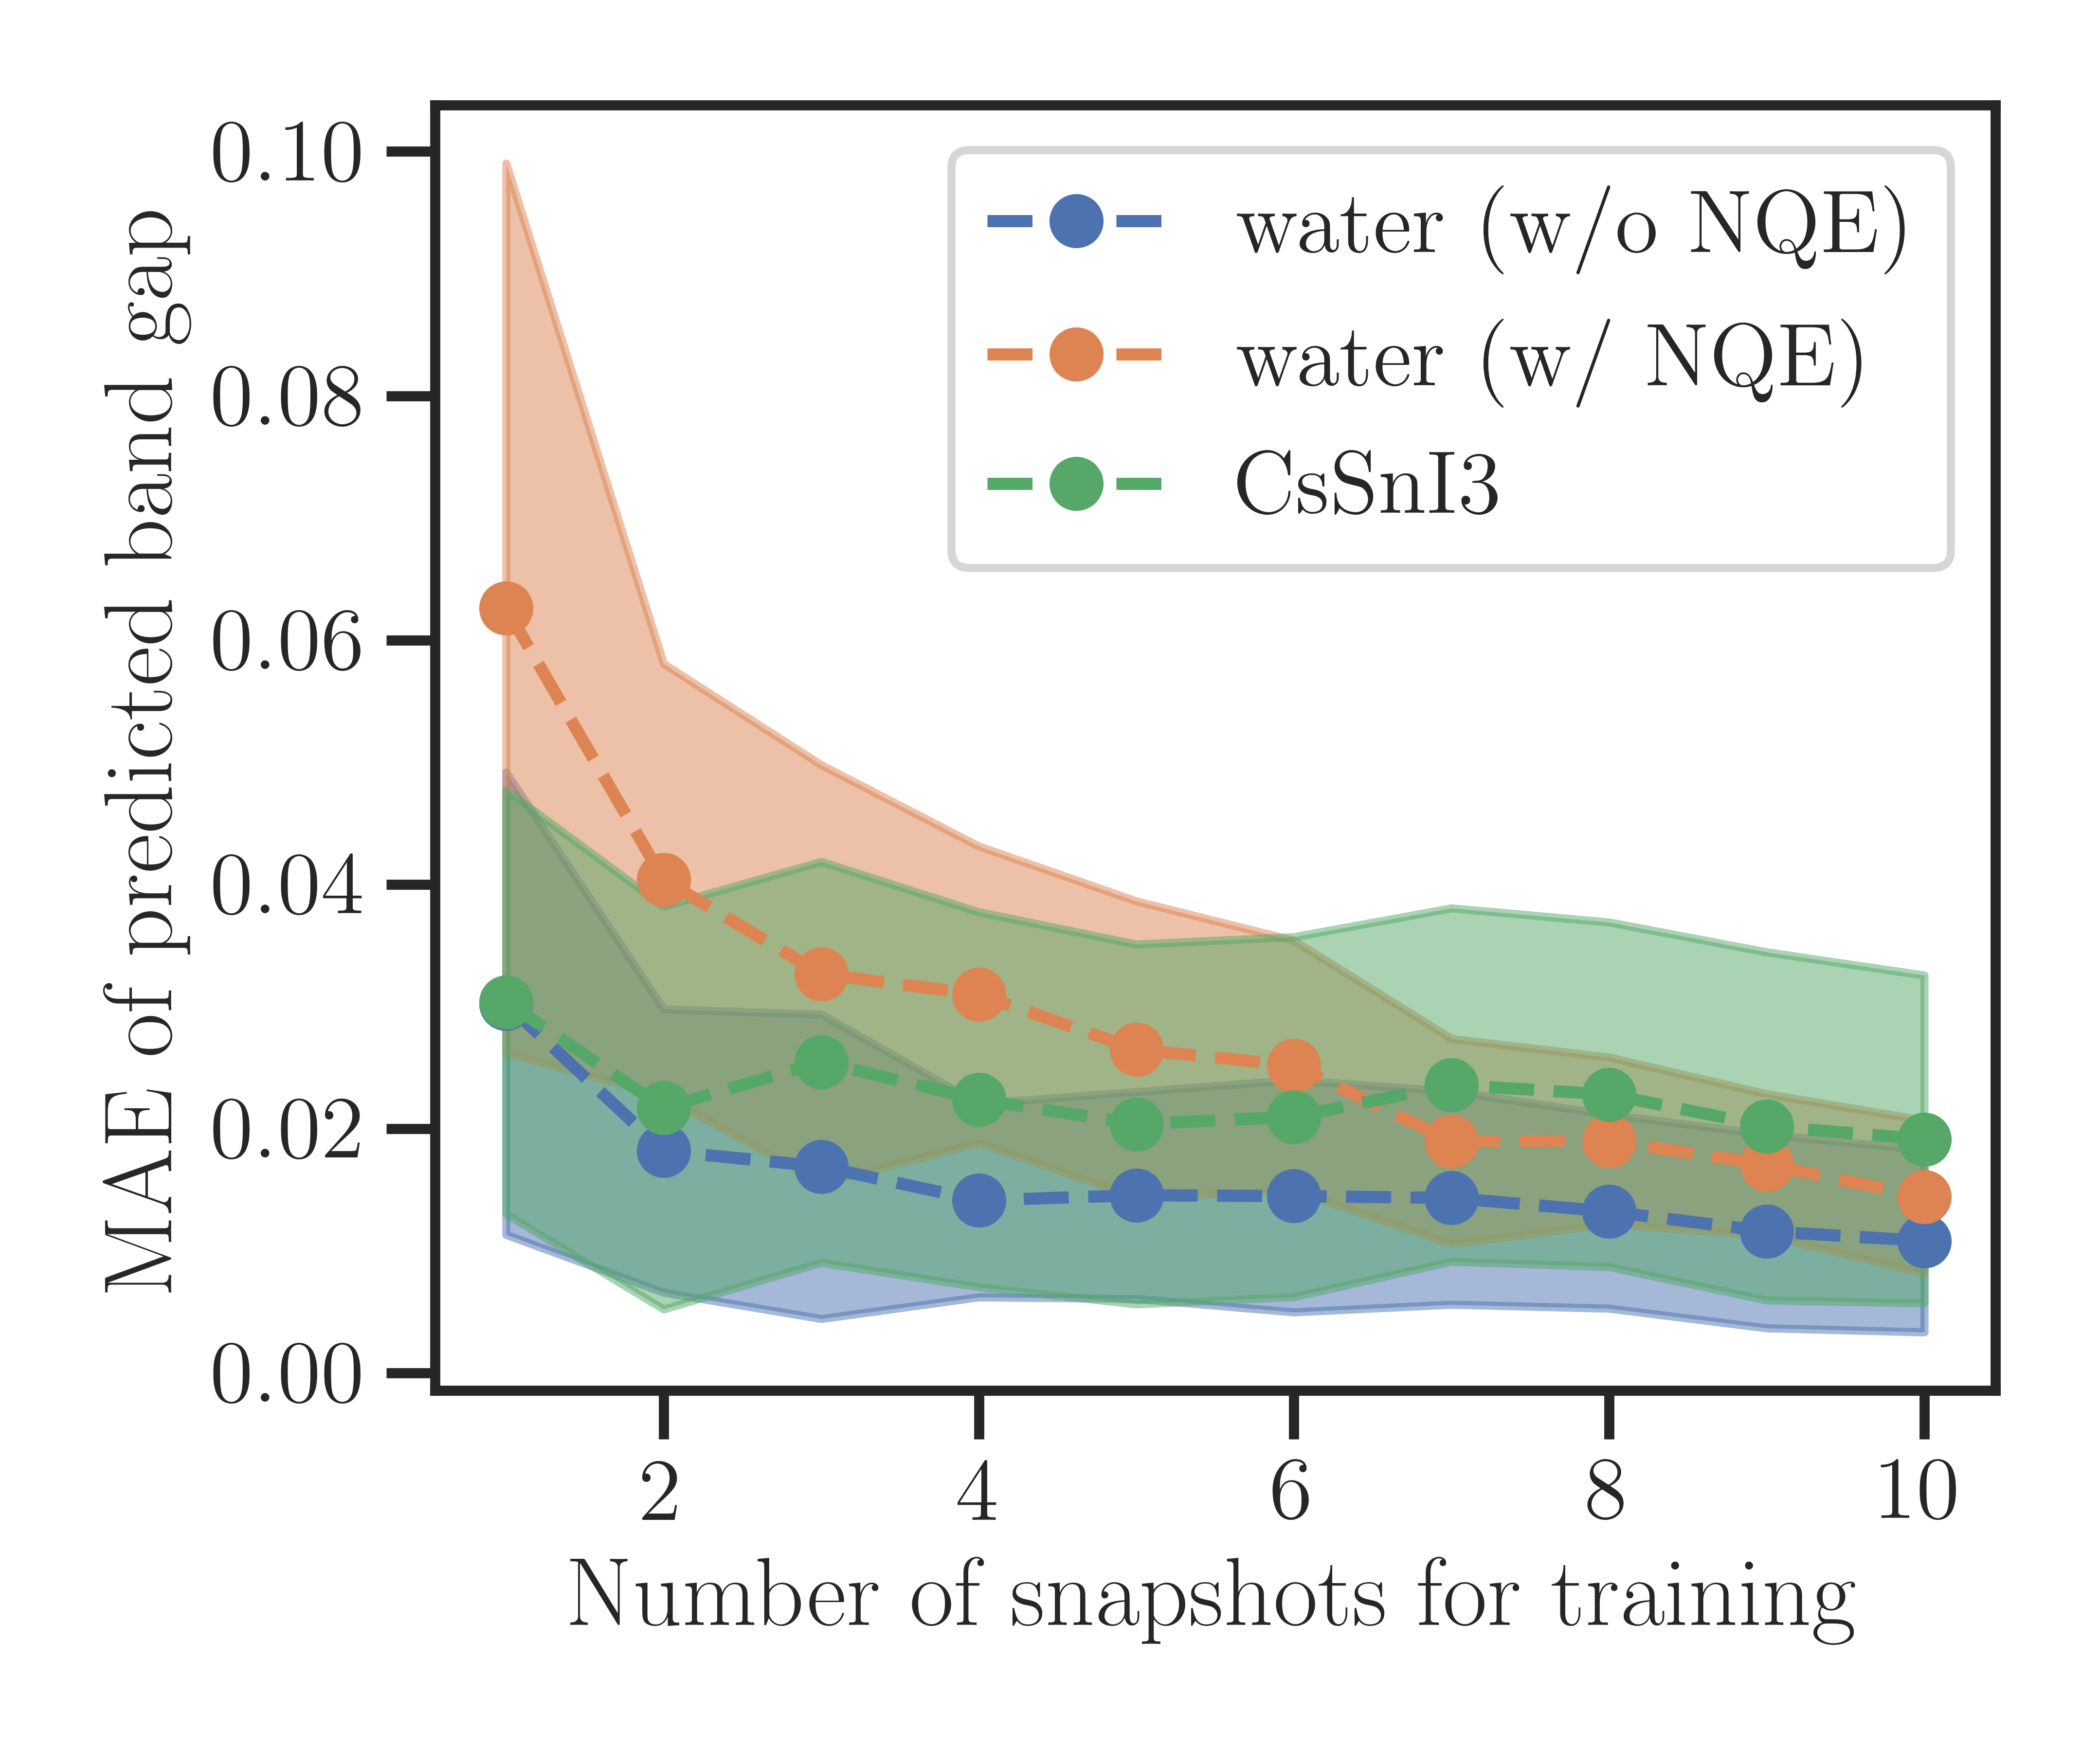
\includegraphics[height=0.7\paperheight]{figures/convergence_analysis_Edward.png}
% 
%       loss of accuracy of the band gap of $\sim$ 0.02 eV
% 
%       (cf. when calculating screening parameters \emph{ab initio})
% 
%       speedup of 70$\times$
%    \end{center}
% 
%    \blfootcite{Schubert2022}
% 
% \end{frame}


\backupend
\end{document}